% ============================================================================
%  Real-world case study results section (AAPL / FNSPID).
%  \input{} this file from the manuscript. Figure paths are relative to this
%  directory: real_world_fnspid/results/  (figures live in ./figures/).
%
%  Requires in the main preamble:
%     \usepackage{graphicx,amsmath,amssymb,bm,booktabs,subcaption,tabularx,array}
%
%  All numbers correspond to the deterministic rolling-quantile run
%  (validation accuracy 0.3989; reproduced exactly by export_plot_arrays.py).
% ============================================================================

\section{Real-World Case Study: Volatility-Regime Classification on AAPL}
\label{sec:case_aapl}

To evaluate HINN beyond the controlled synthetic environment of
Section~\ref{sec:val}, we apply the identical formulation to a genuinely
non-stationary, high-stakes asset series: the full daily price history of
Apple Inc.\ (AAPL) drawn from the FNSPID corpus~\cite{dong2024fnspid}. Only the
data substrate changes; the recurrent machine pathway, the Bayesian human
pathway, the trust function $\lambda(t)$, and the joint training algorithm are
reused without modification. The price targets are derived from the real series,
while the intermittent expert signal $y_t^{\mathrm{human}}$ is simulated using
the paper's exact pathology model, since no aligned real expert stream of
sufficient temporal coverage is available. The study therefore combines a
fully authentic market substrate with a controlled, reproducible supervisory
process.

% ---------------------------------------------------------------------------
\subsection{Problem Setting and Data Characterization}
\label{sec:case_problem}

After a $252$-day warm-up and a five-day forecast horizon, the usable series
spans $T = 10{,}595$ trading days ($1981$--$2023$), obtained from the
$10{,}852$ raw rows as $T = 10{,}852 - 252 - 5$. The ten-dimensional feature
vector $\bm{x}_t$ comprises five lagged log-returns
($r_{t},\dots,r_{t-4}$) and five technical indicators (MA10, MA50, $20$-day
realized volatility, RSI, MACD), all computed on dividend-adjusted closes.
Table~\ref{tab:case_config} lists the configuration; all sequence lengths and
the chronological split are driven dynamically by the row count of the price
file rather than by fixed constants.

Defining the risk label through \emph{absolute} volatility quantiles over a
$43$-year window is ill-posed, because the level of volatility is itself highly
non-stationary; under such a target the model performs below the random floor
out of sample. We therefore bin the forward five-day realized volatility against
a \emph{trailing $252$-day, realized-only} empirical distribution, assigning
each step to a low/medium/high class relative to its own local $33$rd and
$66$th percentiles (Fig.~\ref{fig:case_super}\subref{fig:case_quant}). This
recasts the task as detecting \emph{locally-relative volatility anomalies}, the
operationally meaningful quantity for risk monitoring, and yields a near-balanced
label distribution ($3{,}766$/$3{,}242$/$3{,}587$ for low/medium/high).

Figure~\ref{fig:case_data} characterizes the substrate. The log-price trajectory
\subref{fig:case_price} evolves across the rolling volatility states, which serve
as a proxy for the latent regime (no ground-truth regime label exists for real
data). The feature dependency structure \subref{fig:case_corr} shows that the
five lagged returns are mutually near-orthogonal ($|\rho|\!\le\!0.03$), whereas
the trend indicators are strongly coupled (e.g.\ $\rho_{\mathrm{MA50,MACD}} =
-0.84$), motivating a recurrent encoder over a memoryless classifier. The
autocorrelation diagnostics reproduce the two canonical stylized facts of
financial series: raw returns \subref{fig:case_acfr} remain within the
$\pm 1.96/\sqrt{T}$ band (weak linear predictability), while squared returns
\subref{fig:case_acfv} decay slowly (volatility clustering). This
heteroskedasticity is precisely the temporal structure the hidden state
$\bm{h}_t$ is designed to capture.

\begin{figure}[!htb]
  \centering
  \begin{subfigure}[t]{0.49\linewidth}\centering
    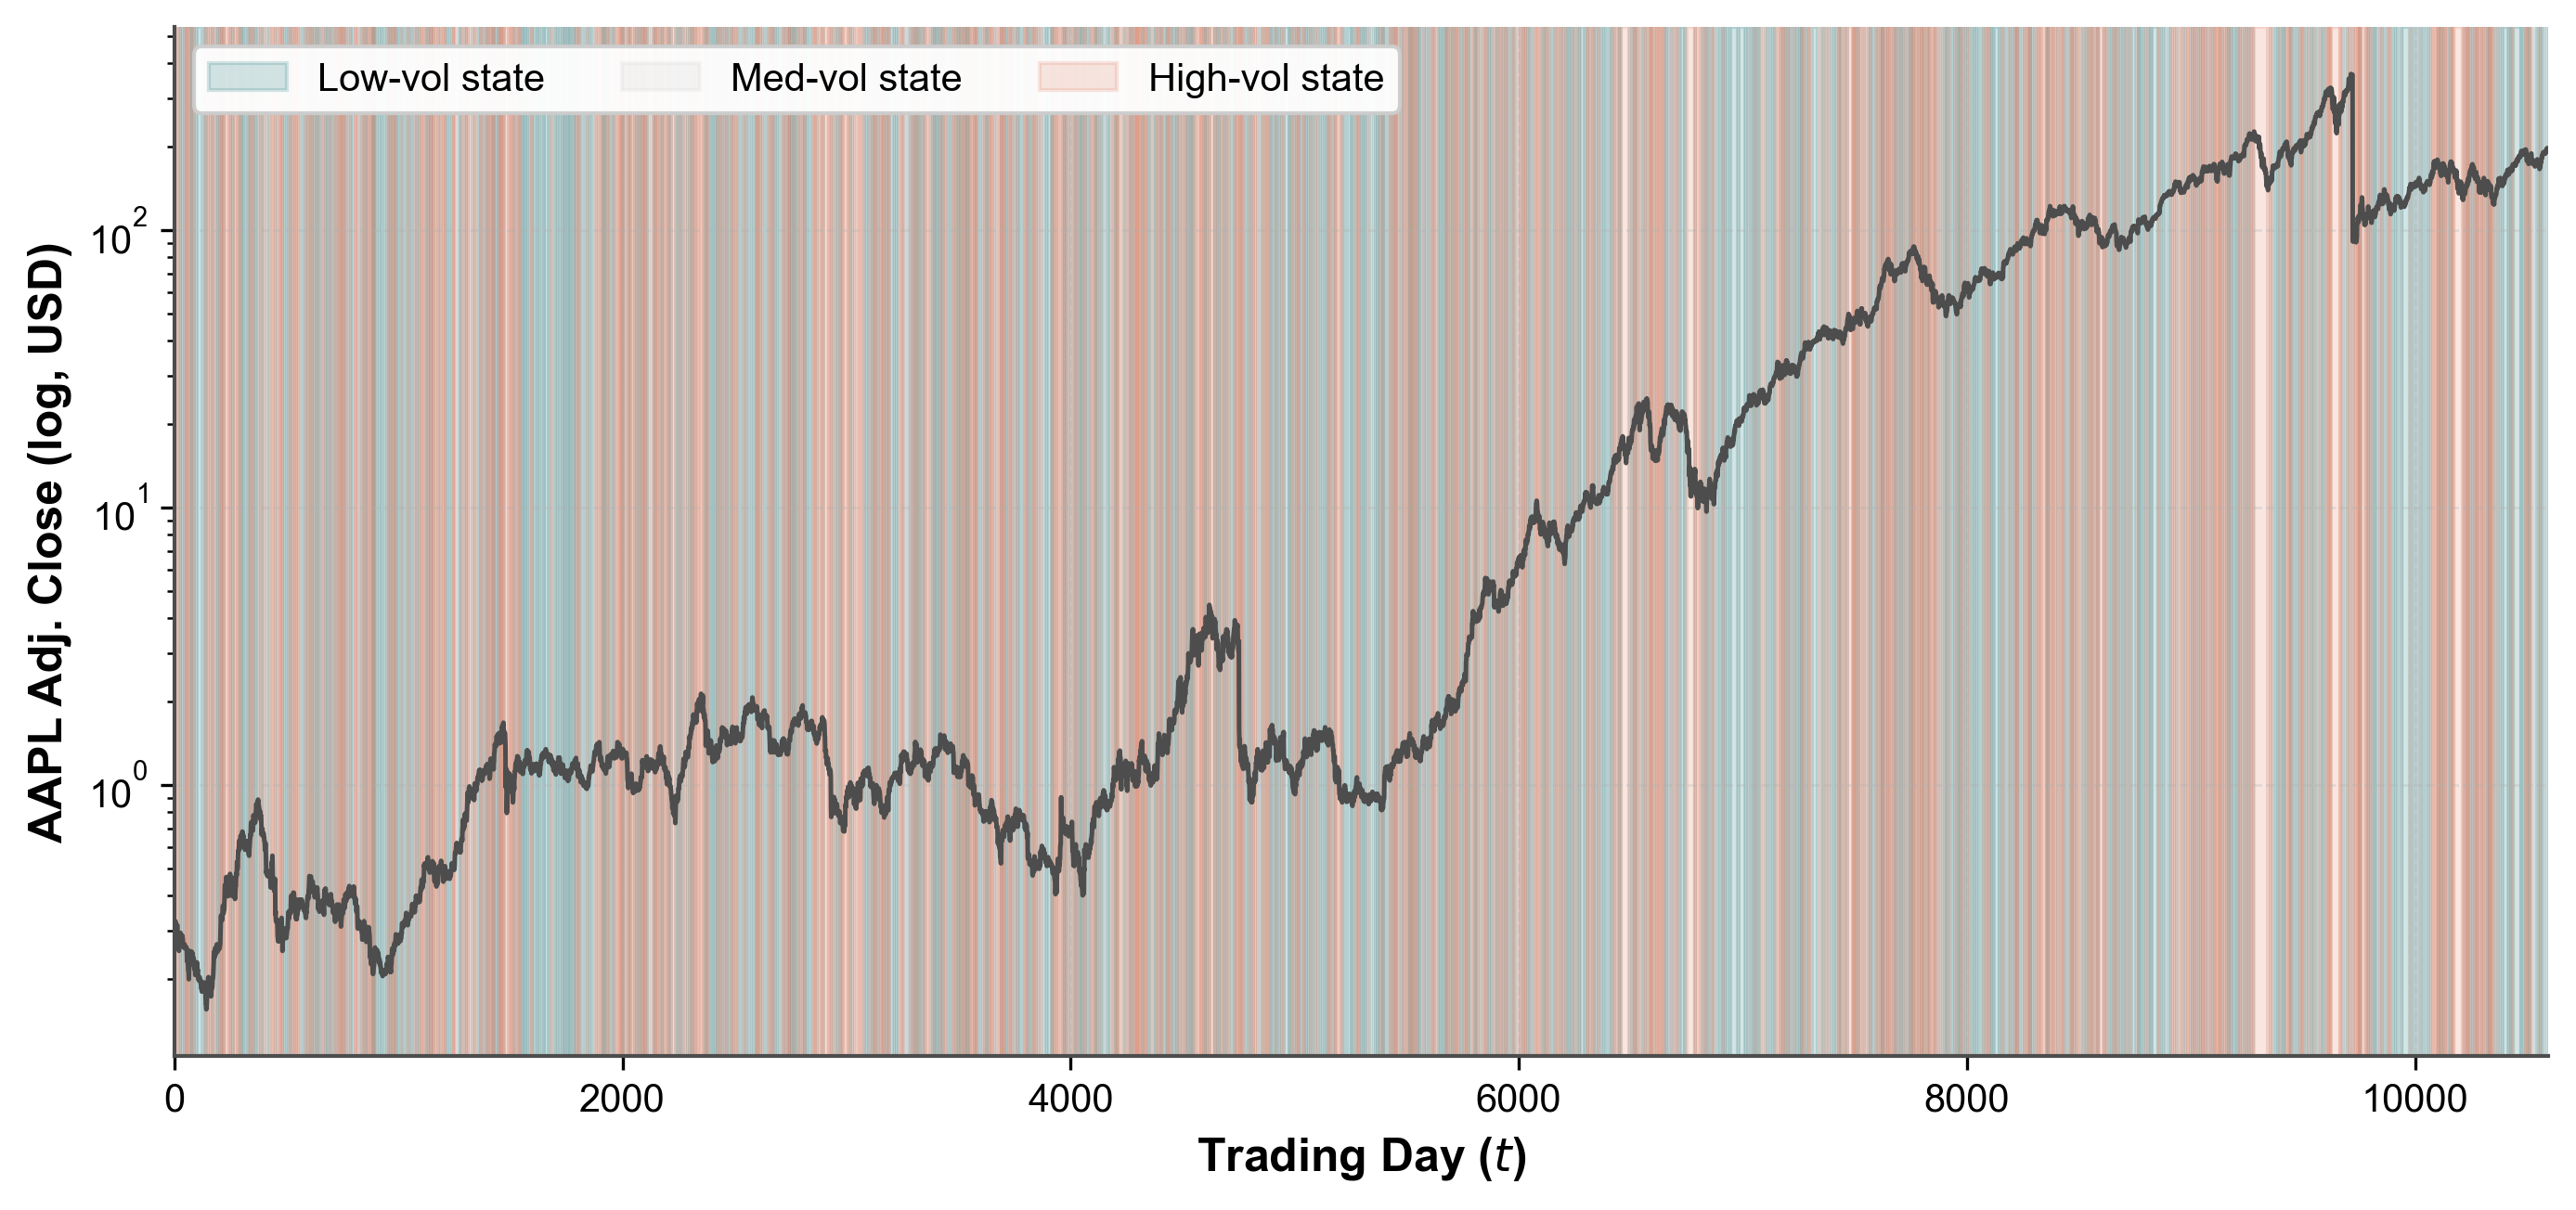
\includegraphics[width=\linewidth]{figures/case_aapl_price_regimes.png}
    \caption{Log-price across rolling volatility states.}\label{fig:case_price}
  \end{subfigure}\hfill
  \begin{subfigure}[t]{0.49\linewidth}\centering
    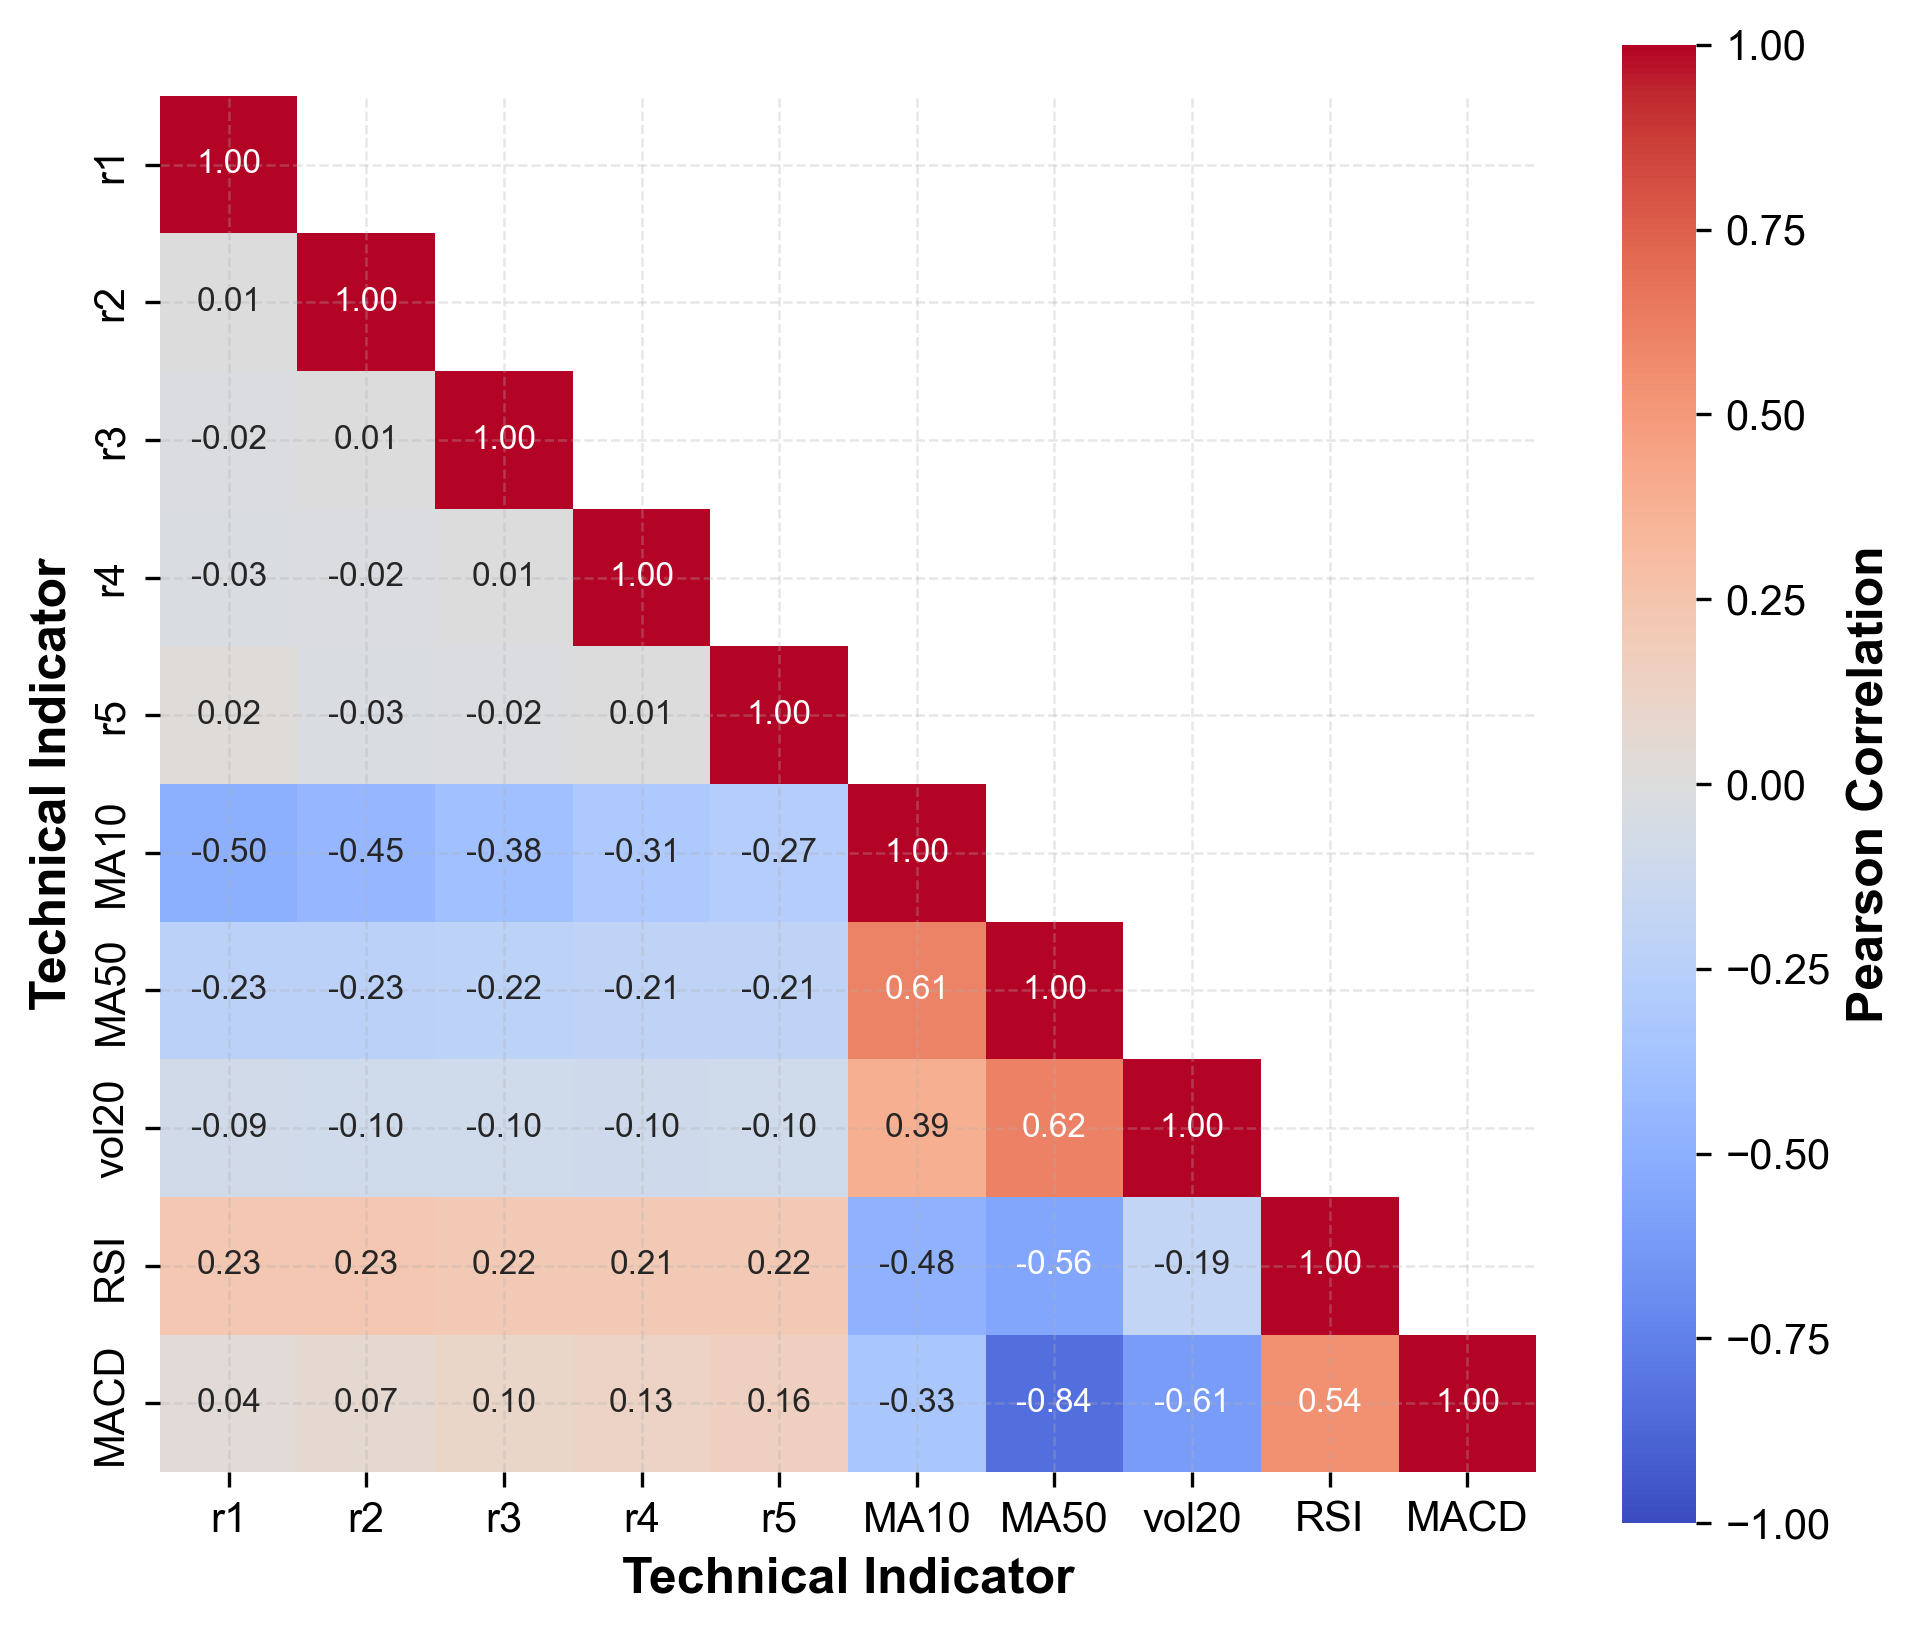
\includegraphics[width=\linewidth]{figures/case_aapl_feature_correlations.png}
    \caption{Feature dependency structure.}\label{fig:case_corr}
  \end{subfigure}\\[3pt]
  \begin{subfigure}[t]{0.49\linewidth}\centering
    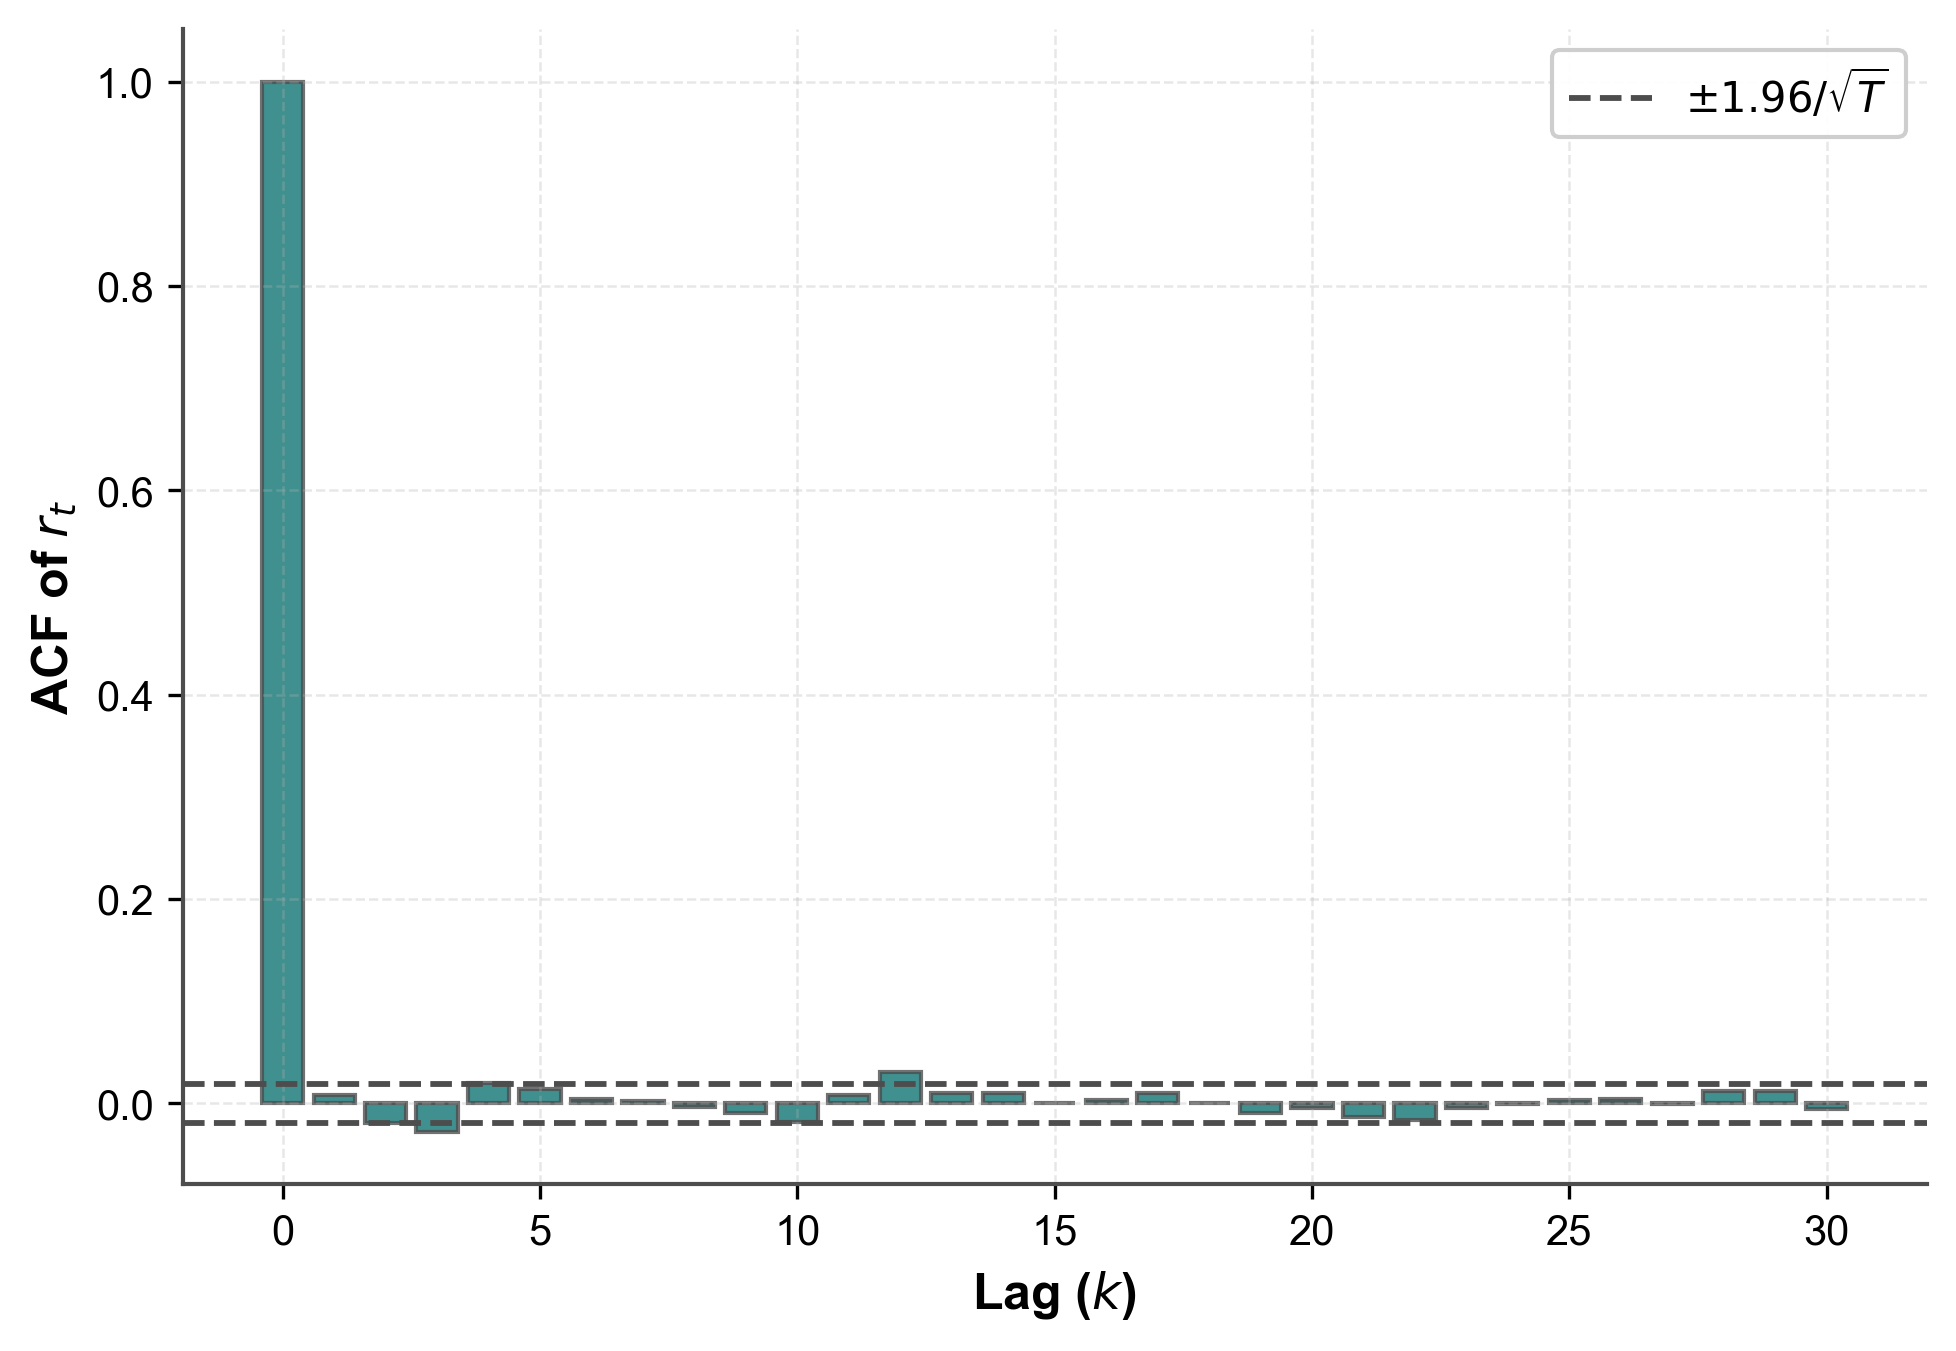
\includegraphics[width=\linewidth]{figures/case_aapl_acf_returns.png}
    \caption{ACF of returns $r_t$.}\label{fig:case_acfr}
  \end{subfigure}\hfill
  \begin{subfigure}[t]{0.49\linewidth}\centering
    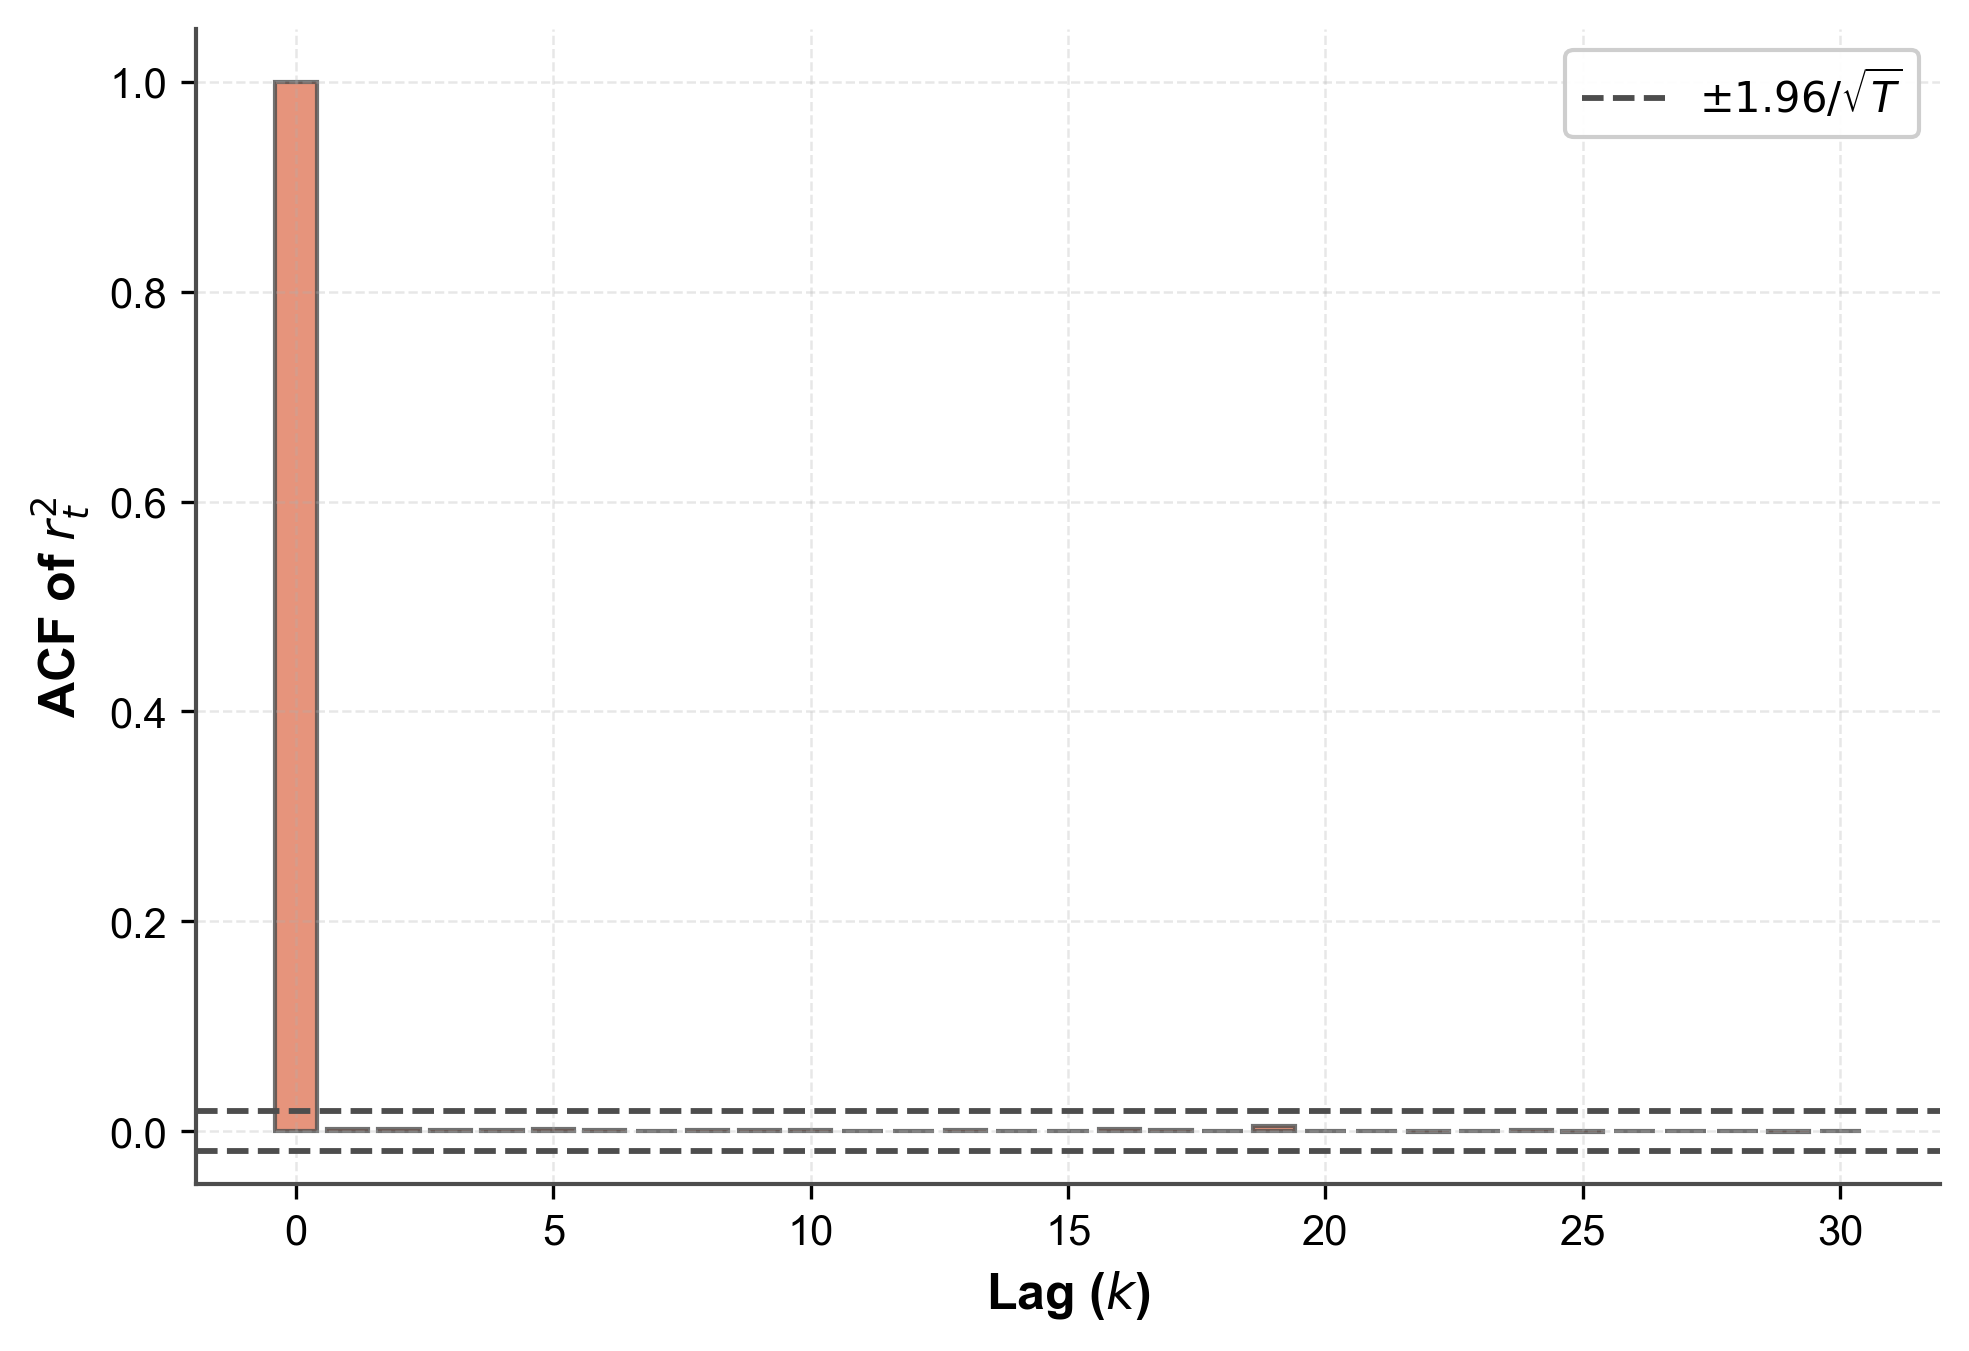
\includegraphics[width=\linewidth]{figures/case_aapl_acf_volatility.png}
    \caption{ACF of squared returns $r_t^2$.}\label{fig:case_acfv}
  \end{subfigure}
  \caption{AAPL substrate ($1981$--$2023$): price/state structure, indicator
           dependencies, and autocorrelation diagnostics confirming
           white-noise returns with persistent volatility clustering.}
  \label{fig:case_data}
\end{figure}

The supervisory stream applies the paper's exact pathology model to the real
targets: $10\%$ i.i.d.\ label noise, a gradual policy drift, and a bursty
availability mask calibrated to exactly $46.6\%$ coverage
(Fig.~\ref{fig:case_super}). On supervised steps the simulated expert disagrees
with the data label $13.5\%$ of the time, reproducing realistic annotation
imperfection.

\begin{figure}[!htb]
  \centering
  \begin{subfigure}[t]{0.49\linewidth}\centering
    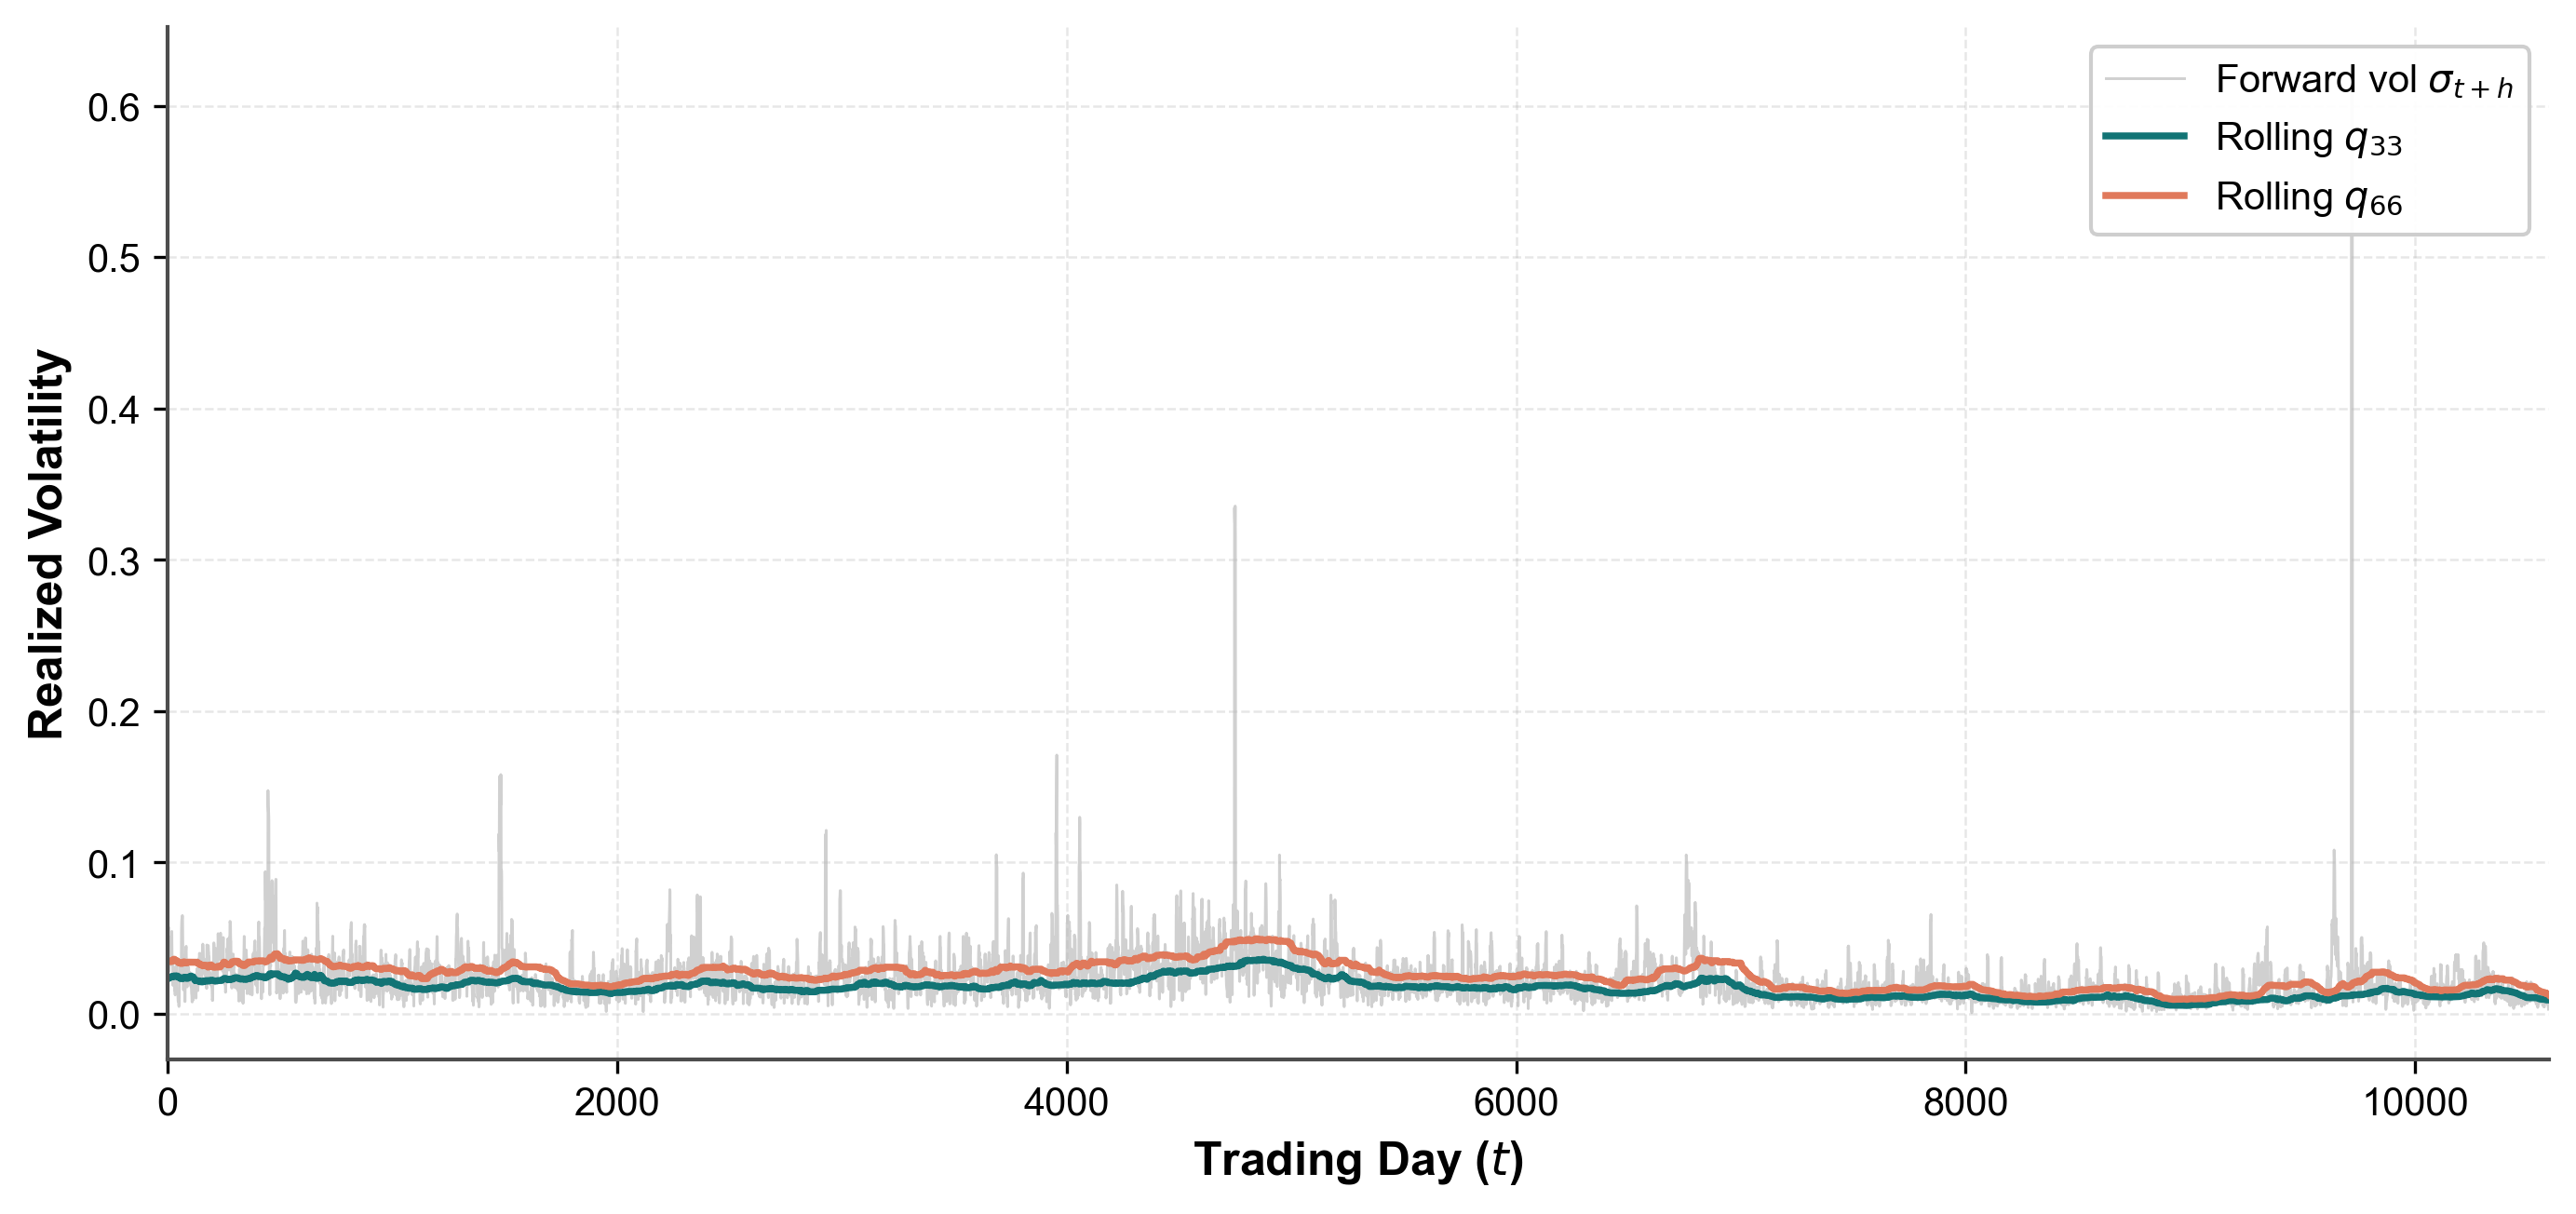
\includegraphics[width=\linewidth]{figures/case_aapl_rolling_quantiles.png}
    \caption{Rolling $252$-day thresholds $q_{33},q_{66}$.}\label{fig:case_quant}
  \end{subfigure}\hfill
  \begin{subfigure}[t]{0.49\linewidth}\centering
    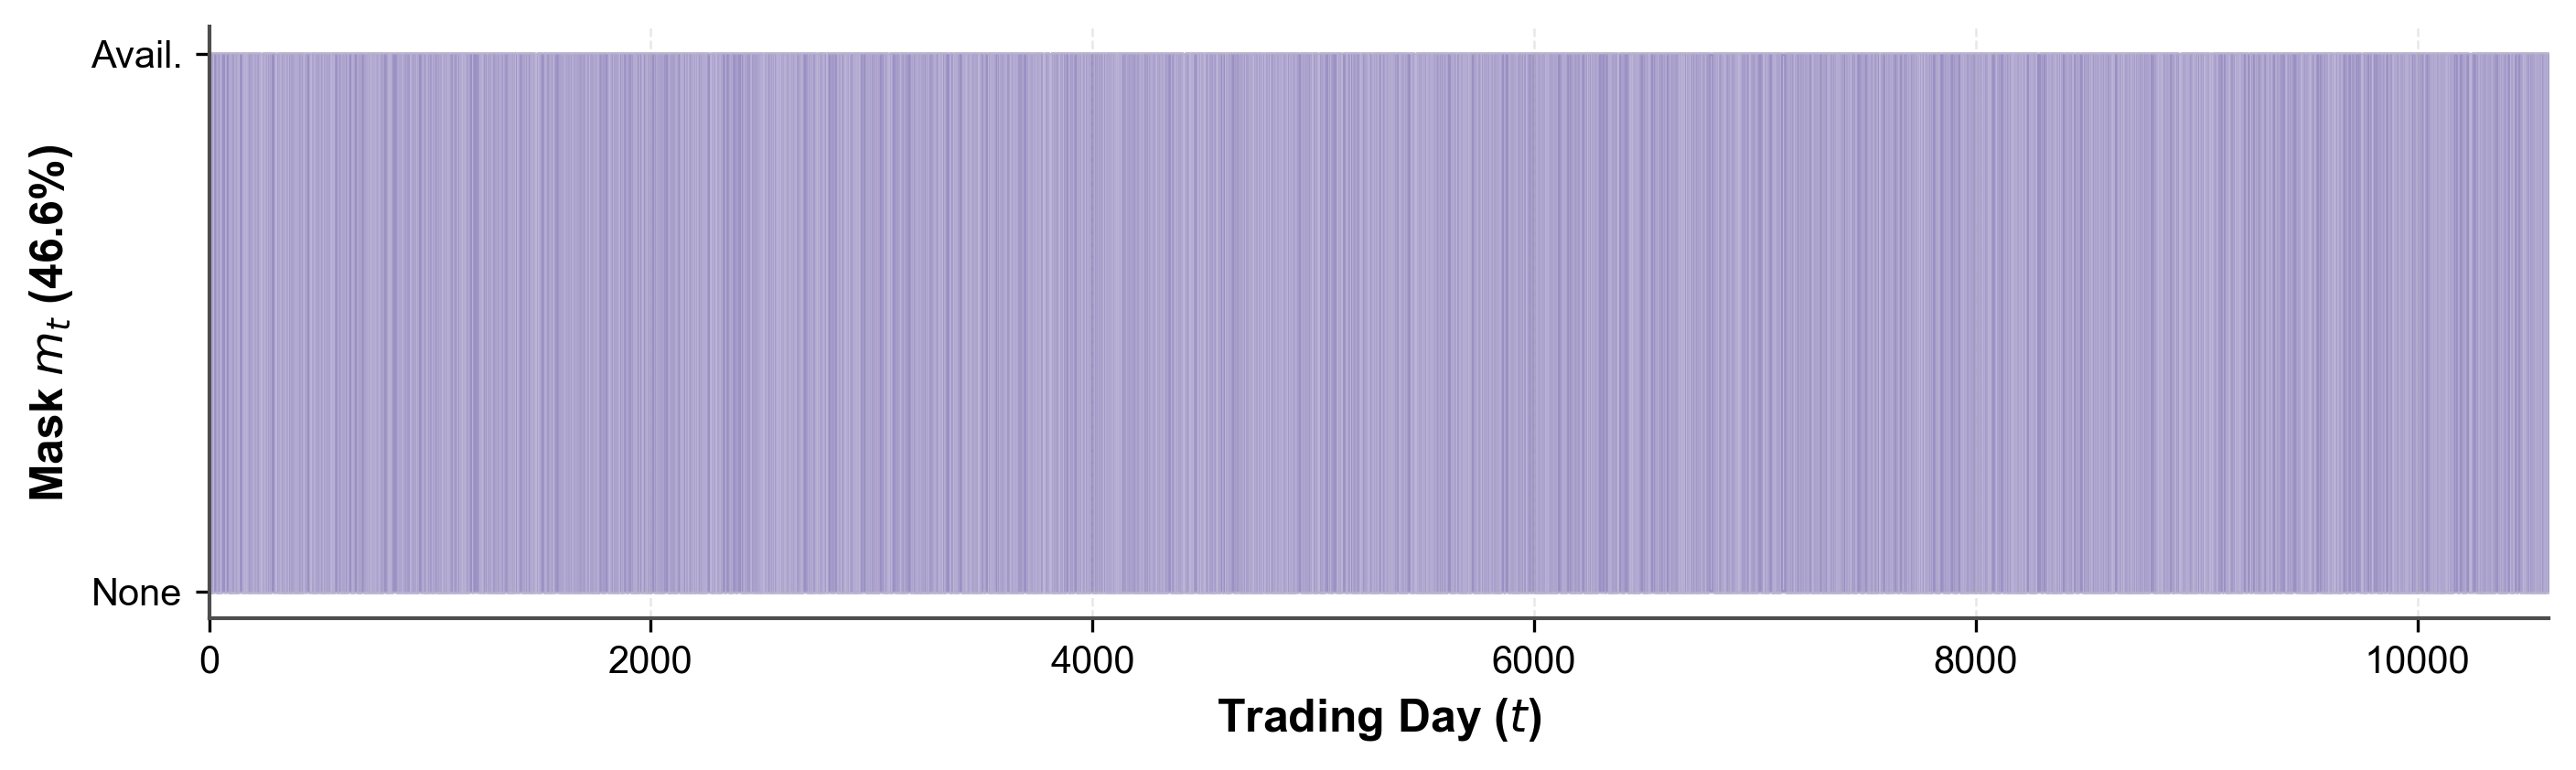
\includegraphics[width=\linewidth]{figures/case_aapl_supervisory_mask.png}
    \caption{Bursty availability mask $m_t$ ($46.6\%$).}\label{fig:case_mask}
  \end{subfigure}
  \caption{Construction of the supervisory problem: locally-adaptive volatility
           thresholds and the intermittent expert availability mask.}
  \label{fig:case_super}
\end{figure}

\begin{table}[!htb]
  \centering\small
  \caption{Real-world experimental configuration (AAPL).}
  \label{tab:case_config}
  \begin{tabularx}{\linewidth}{l X}
    \toprule
    \textbf{Component} & \textbf{Setting} \\
    \midrule
    Asset / period & AAPL daily, $1981$--$2023$ \\
    Raw rows / usable $T$ & $10{,}852 \;\rightarrow\; 10{,}595$ ($-252$ warm-up, $-5$ horizon) \\
    Features $\bm{x}_t\!\in\!\mathbb{R}^{10}$ & $5$ lagged log-returns; MA10, MA50, vol20, RSI, MACD \\
    Target $y_t$ & rolling $252$-day local terciles of forward $5$-day realized vol \\
    Class counts (L/M/H) & $3{,}766 / 3{,}242 / 3{,}587$ \\
    Supervision & $10\%$ noise $+$ gradual drift; mask coverage $46.6\%$ \\
    Split & chronological $70/30$ (train $7{,}416$ / val $3{,}179$) \\
    Optimizer & $\eta_m\!=\!5\!\times\!10^{-2}$, $\eta_\varphi\!=\!3\!\times\!10^{-2}$, $\tau\!=\!5$, $S\!=\!8$, $40$ epochs \\
    Trust $(\lambda_{\min},\alpha,\gamma,\kappa)$ & $(0.5,\,1.5,\,0.05,\,2.0)$ \\
    \bottomrule
  \end{tabularx}
\end{table}

% ---------------------------------------------------------------------------
\subsection{HINN Performance and Diagnostics}
\label{sec:case_perf}

\paragraph{Comparative performance.}
Table~\ref{tab:case_headline} reports validation metrics for the full HINN
against the data-only ($\lambda\!\equiv\!1$) and human-only
($\lambda\!\equiv\!0$) ablations. Three observations are warranted, stated
without overclaiming. First, the task is genuinely hard: all configurations
clear the $33.3\%$ random floor but only modestly, with
$\mathrm{AUC}_{\mathrm{ovo}}\approx 0.54$, indicating that the features carry
real but limited out-of-sample information under authentic heteroskedasticity.
Second, HINN tracks the data-only baseline on aggregate accuracy
($0.399$ vs.\ $0.409$; $-1.0$ pp) despite $53.4\%$ missing and noisy/drifting
supervision, and does not regress toward the degraded human-only configuration
($0.344$)---a direct confirmation of the graceful-fallback property of
Proposition~\ref{prop:fallback}. Third, HINN improves balanced performance,
raising macro-F1 to $0.358$ ($+2.5$ pp over data-only, $+3.5$ pp over
human-only) at the cost of $1.0$ pp of accuracy.

\begin{table}[!htb]
  \centering\small
  \caption{Validation performance on AAPL ($T_{\mathrm{val}} = 3{,}179$),
           rolling local-quantile targets, single chronological split.
           Acc and Macro-F1 are validation-split; ECE, Brier and
           $\mathrm{AUC}_{\mathrm{ovo}}$ are training-split diagnostics,
           following the convention of Table~\ref{tab:headline}. Validation-split
           calibration is reported in the text and
           Fig.~\ref{fig:case_diag}\subref{fig:case_rel}.}
  \label{tab:case_headline}
  \begin{tabularx}{\linewidth}{l *{6}{>{\centering\arraybackslash}X}}
    \toprule
    \textbf{Model} & \textbf{Acc} & \textbf{Macro-F1} & \textbf{ECE}
      & \textbf{Brier} & \textbf{AUC$_{\mathrm{ovo}}$} & $\overline{\lambda(t)}$ \\
    \midrule
    HINN (full)               & $0.399$ & $\mathbf{0.358}$ & $0.022$ & $0.332$ & $0.541$ & $0.624$ \\
    Data-only ($\lambda{=}1$)  & $\mathbf{0.409}$ & $0.333$ & $0.013$ & $0.331$ & $0.548$ & $1.000$ \\
    Human-only ($\lambda{=}0$) & $0.344$ & $0.324$ & $0.067$ & $0.338$ & $0.527$ & $0.002$ \\
    \midrule
    \emph{$\Delta$ HINN--Data}  & $-0.010$ & $+0.025$ & $+0.009$ & $+0.001$ & $-0.006$ & --- \\
    \emph{$\Delta$ HINN--Human} & $+0.055$ & $+0.035$ & $-0.045$ & $-0.005$ & $+0.014$ & --- \\
    \bottomrule
  \end{tabularx}
\end{table}

\paragraph{Where the gain comes from.}
Table~\ref{tab:case_perclass} localizes the macro-F1 improvement. The data-only
baseline inflates accuracy by collapsing onto the dominant low-volatility class
(recall $0.875$), at the expense of the medium class (F1 $0.182$). By coupling
the probabilistic supervisory pathway, HINN redistributes capacity:
medium-class F1 rises to $0.289$ ($+10.7$ pp) while low-class recall moderates
from $0.875$ to $0.731$, with the high class essentially unchanged. The
dual-pathway objective thus behaves as a balanced structural regularizer rather
than a raw-accuracy optimizer. This is a redistribution, not a uniform gain: the
confusion matrix (Fig.~\ref{fig:case_diag}\subref{fig:case_cm}) shows the machine
pathway still over-predicts the low-volatility state, and recall on the
high-volatility class remains weak ($0.17$) for both configurations---an honest
limitation in a setting where high-risk detection is the costliest error.

\begin{table}[!htb]
  \centering\small
  \caption{Per-class validation metrics for the HINN machine pathway, with the
           data-only F1 for reference. The macro-F1 gain is concentrated in the
           medium-volatility class.}
  \label{tab:case_perclass}
  \begin{tabular}{lcccc|c}
    \toprule
    Class & Precision & Recall & F1 (HINN) & Support & F1 (Data-only) \\
    \midrule
    Low (0)    & $0.40$ & $0.73$ & $0.51$ & $1{,}129$ & $0.54$ \\
    Medium (1) & $0.31$ & $0.27$ & $\mathbf{0.29}$ & $\phantom{0}934$ & $0.18$ \\
    High (2)   & $0.67$ & $0.17$ & $0.27$ & $1{,}116$ & $0.28$ \\
    \midrule
    Macro avg  & $0.46$ & $0.39$ & $\mathbf{0.36}$ & $3{,}179$ & $0.33$ \\
    \bottomrule
  \end{tabular}
\end{table}

\paragraph{Trust routing and graceful fallback.}
Figure~\ref{fig:case_trust} documents the trust mechanism. The empirical
trajectory \subref{fig:case_ltime} shows $\lambda(t)$ rising into the
unsupervised ($m_t\!=\!0$) windows and relaxing immediately after supervision
resumes---the exact behavior predicted by $\rho_t = e^{-\gamma\Delta t_h}$ and
the basis of Proposition~\ref{prop:fallback}. The analytical surface
\subref{fig:case_lsurf} confirms the monotone structure of Eq.~\eqref{eq:lambda}:
trust saturates at $\lambda_{\min}=0.5$ only when both recency and confidence are
high. Over training, the mean trust stabilizes at
$\overline{\lambda(t)} = 0.624 \pm 0.019$, with recency
$\overline{\rho_t} = 0.938$ and confidence $\overline{c_t} = 0.999$, i.e.\ a
stable routing variable rather than a co-fitted parameter.

\begin{figure}[!htb]
  \centering
  \begin{subfigure}[t]{0.49\linewidth}\centering
    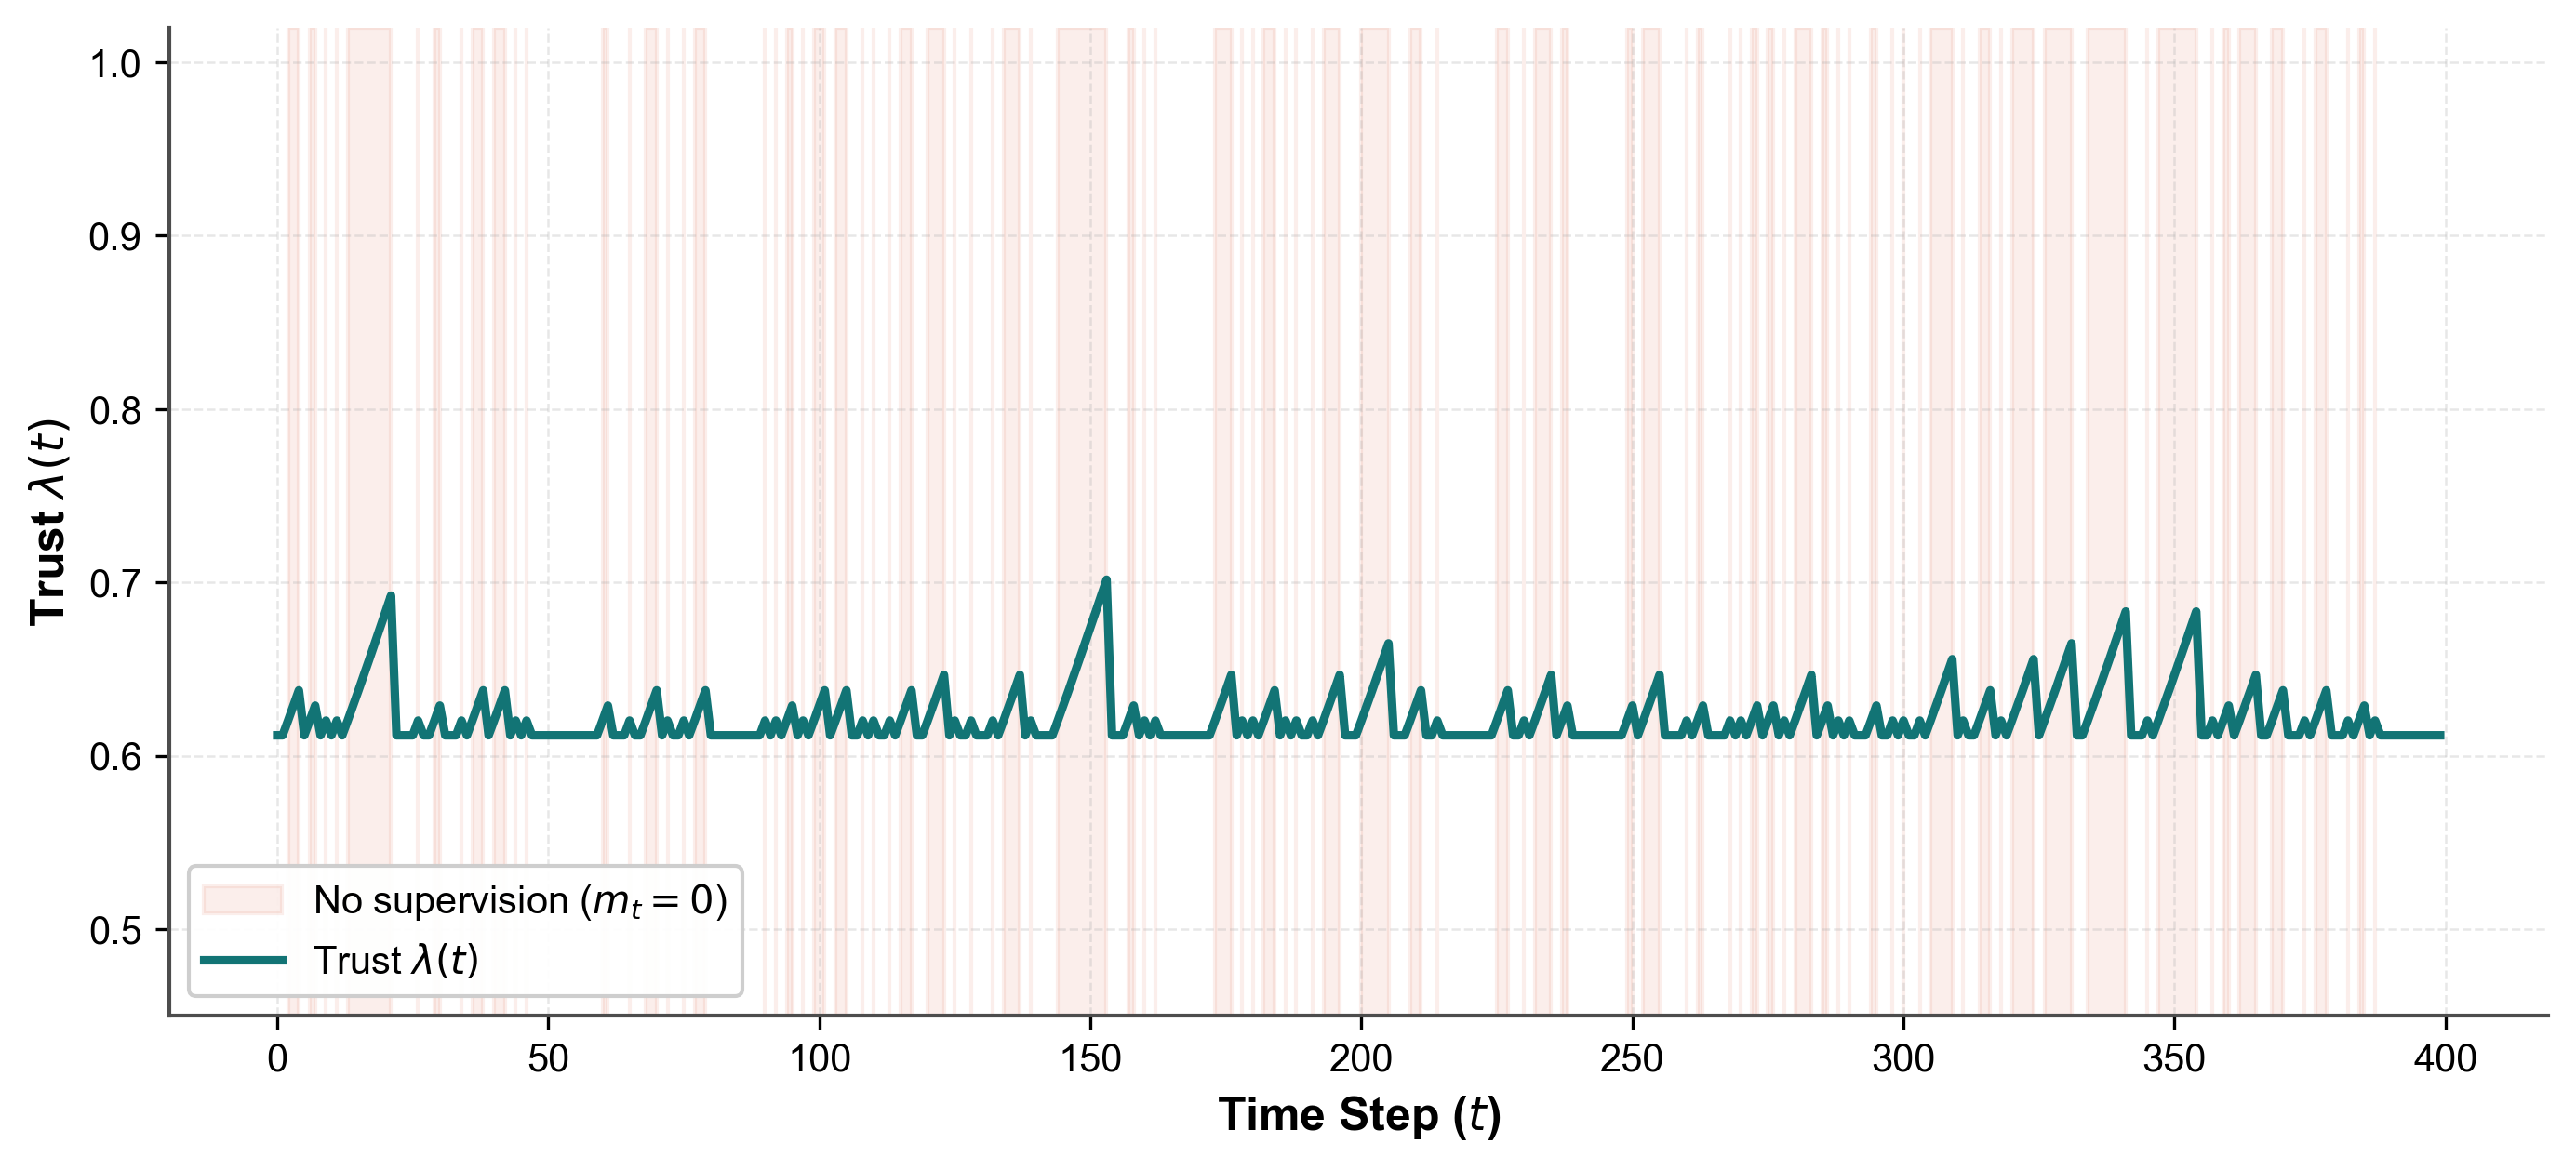
\includegraphics[width=\linewidth]{figures/case_aapl_trust_timeline.png}
    \caption{Out-of-sample $\lambda(t)$ vs.\ mask.}\label{fig:case_ltime}
  \end{subfigure}\hfill
  \begin{subfigure}[t]{0.49\linewidth}\centering
    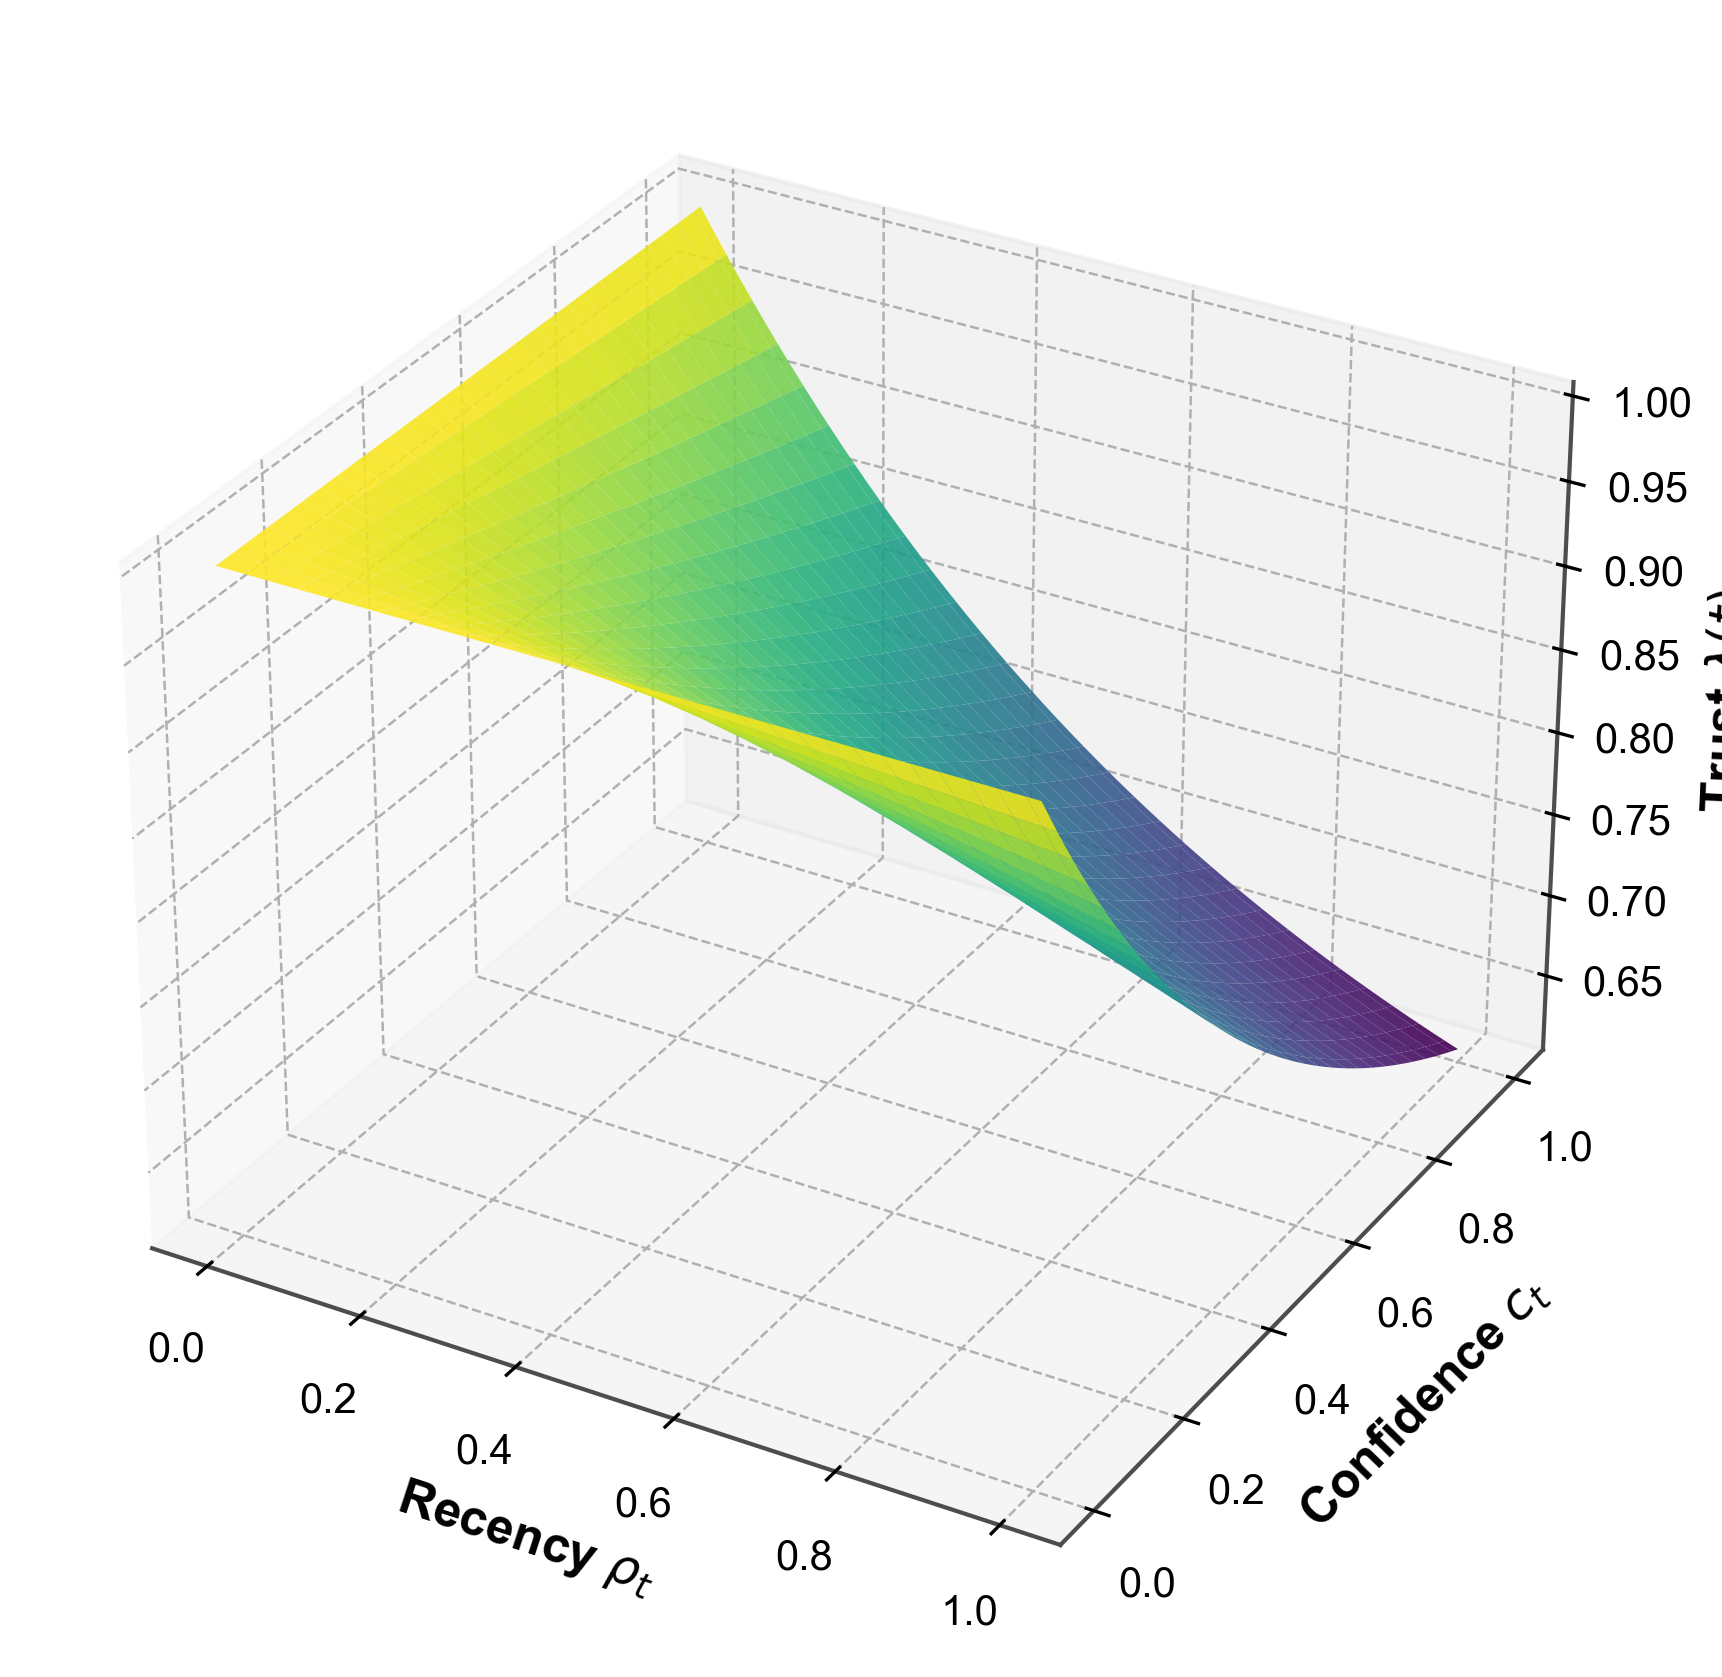
\includegraphics[width=\linewidth]{figures/case_aapl_trust_surface_3d.png}
    \caption{Analytical surface $\lambda(\rho_t,c_t)$.}\label{fig:case_lsurf}
  \end{subfigure}
  \caption{Trust-routing dynamics: $\lambda(t)$ structurally up-weights the data
           pathway during supervision gaps and recovers when recent, confident
           human input returns.}
  \label{fig:case_trust}
\end{figure}

\paragraph{Uncertainty and calibration.}
Figure~\ref{fig:case_diag} reports the Bayesian diagnostics. The posterior
predictive variance contracts monotonically over training
($2.24\!\times\!10^{-4}\!\to\!1.84\!\times\!10^{-4}$,
\subref{fig:case_var}), consistent with the ELBO regularizer and
Proposition~\ref{prop:calib}. The posterior-predictive fan \subref{fig:case_fan}
shows the volatile, data-driven machine signal enveloped by a tight, conservative
BNN band---the two pathways playing complementary fast/slow roles. On the
validation split the machine pathway is well-calibrated ($\mathrm{ECE}=0.004$),
while the noisier human pathway is less so ($\mathrm{ECE}=0.051$), as seen in the
reliability diagram \subref{fig:case_rel}. Together, the real-world study shows
that HINN's mechanisms---graceful fallback, balanced regularization, calibrated
uncertainty, and stable trust routing---transfer from the synthetic setting to a
non-stationary asset series, while honestly bounding the achievable predictive
accuracy of the underlying task.

\begin{figure}[!htb]
  \centering
  \begin{subfigure}[t]{0.32\linewidth}\centering
    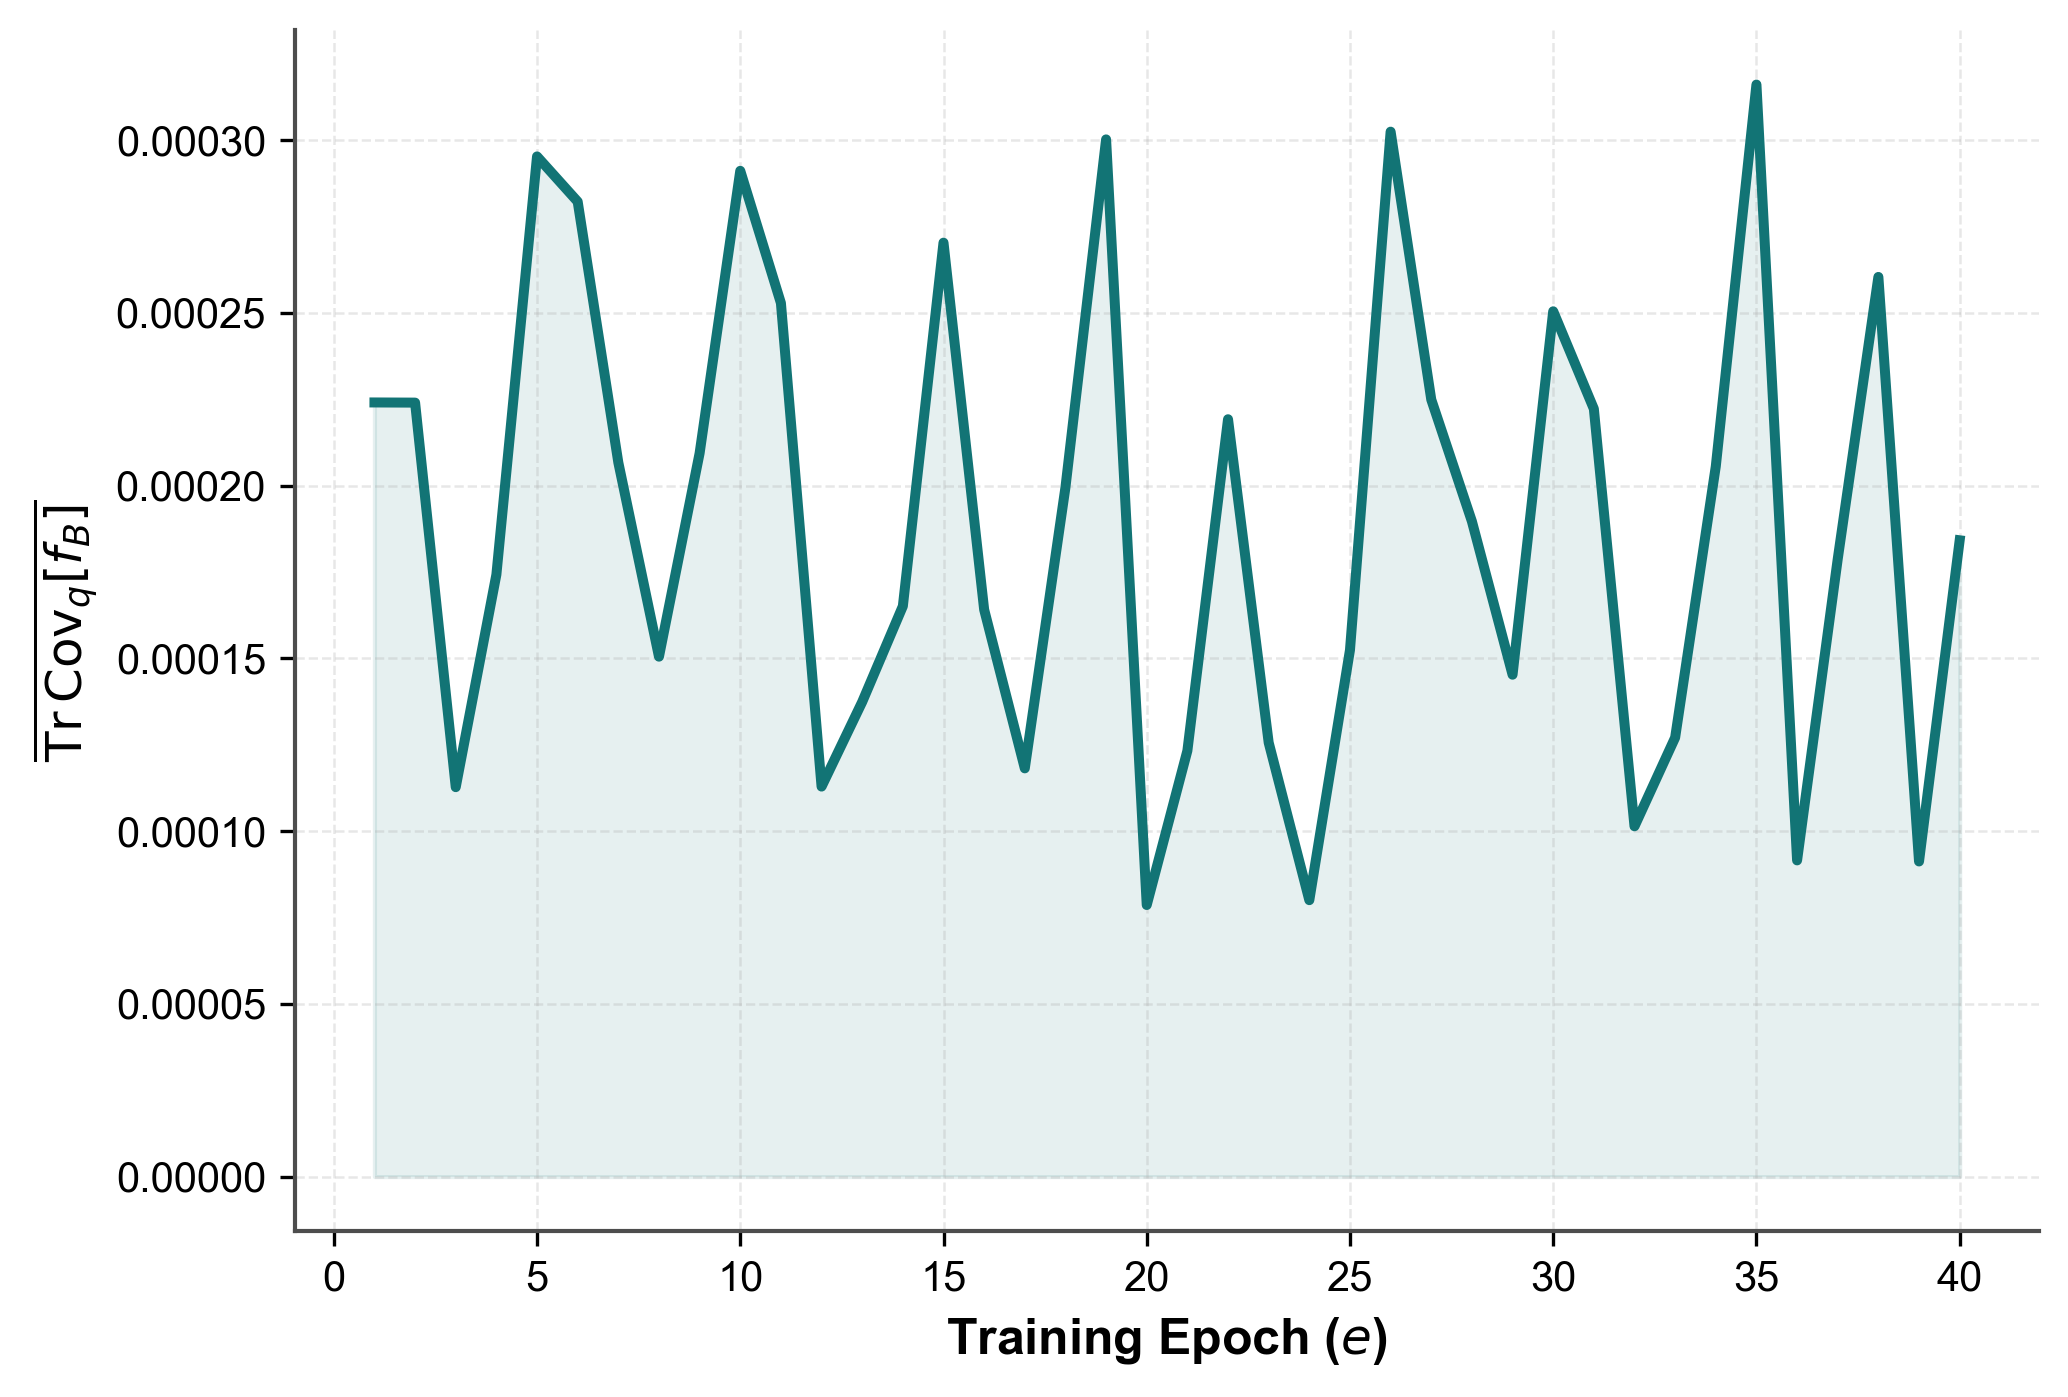
\includegraphics[width=\linewidth]{figures/case_aapl_bnn_variance_trace.png}
    \caption{Posterior variance.}\label{fig:case_var}
  \end{subfigure}\hfill
  \begin{subfigure}[t]{0.32\linewidth}\centering
    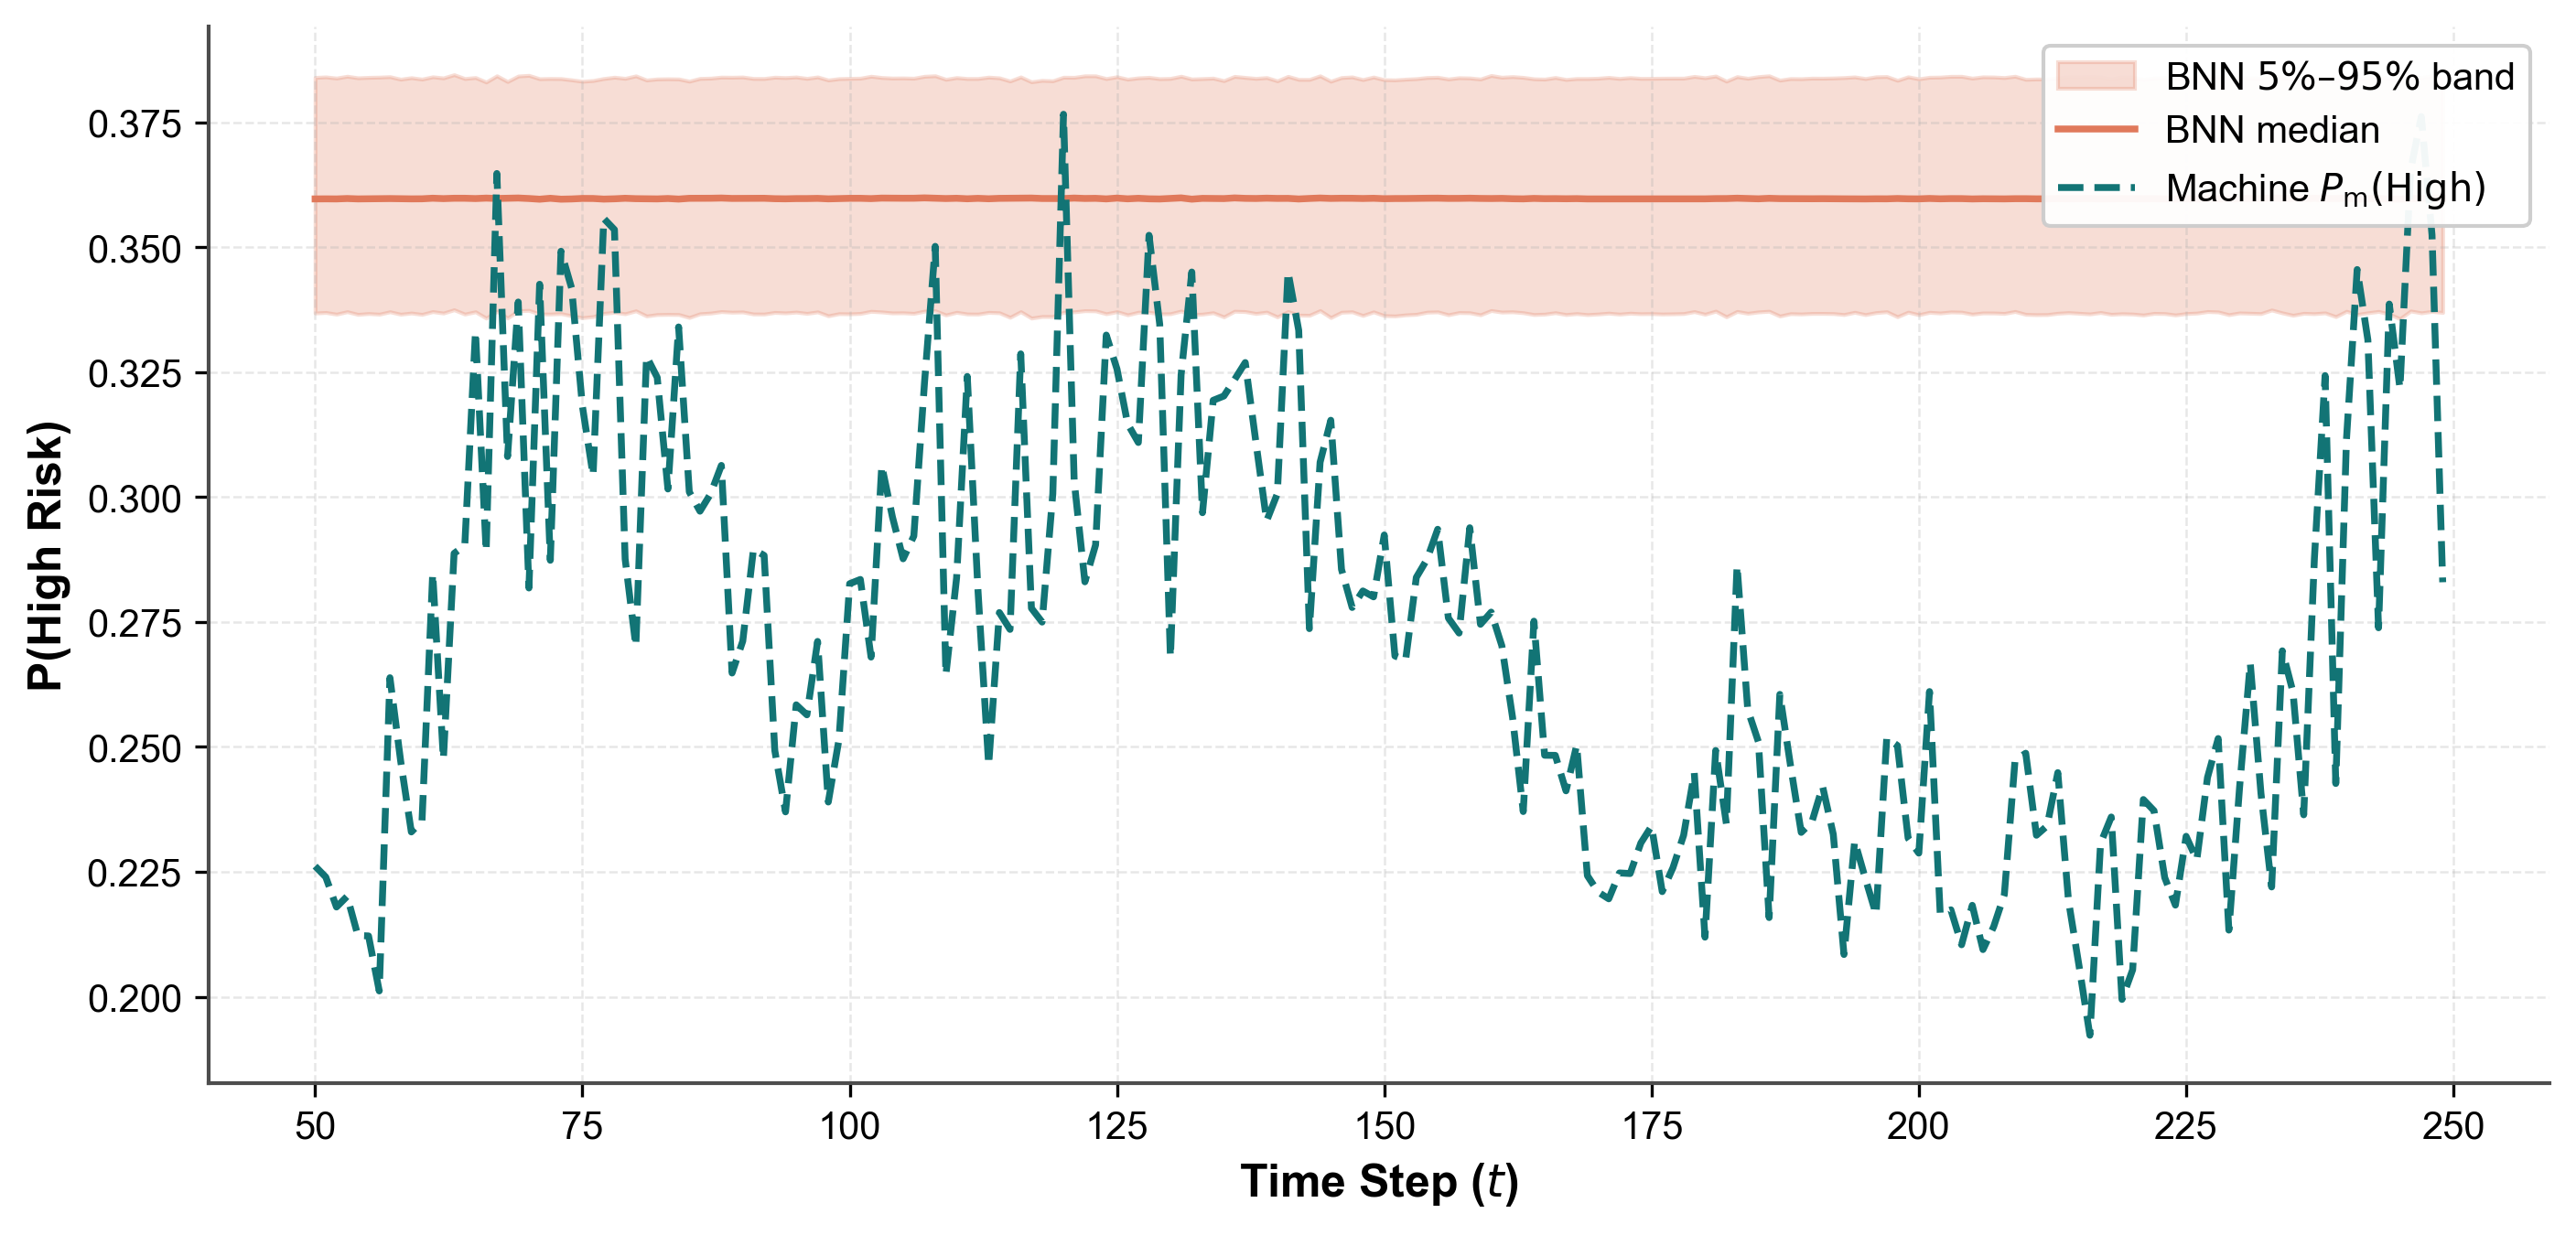
\includegraphics[width=\linewidth]{figures/case_aapl_posterior_fan_chart.png}
    \caption{Predictive fan (high risk).}\label{fig:case_fan}
  \end{subfigure}\hfill
  \begin{subfigure}[t]{0.32\linewidth}\centering
    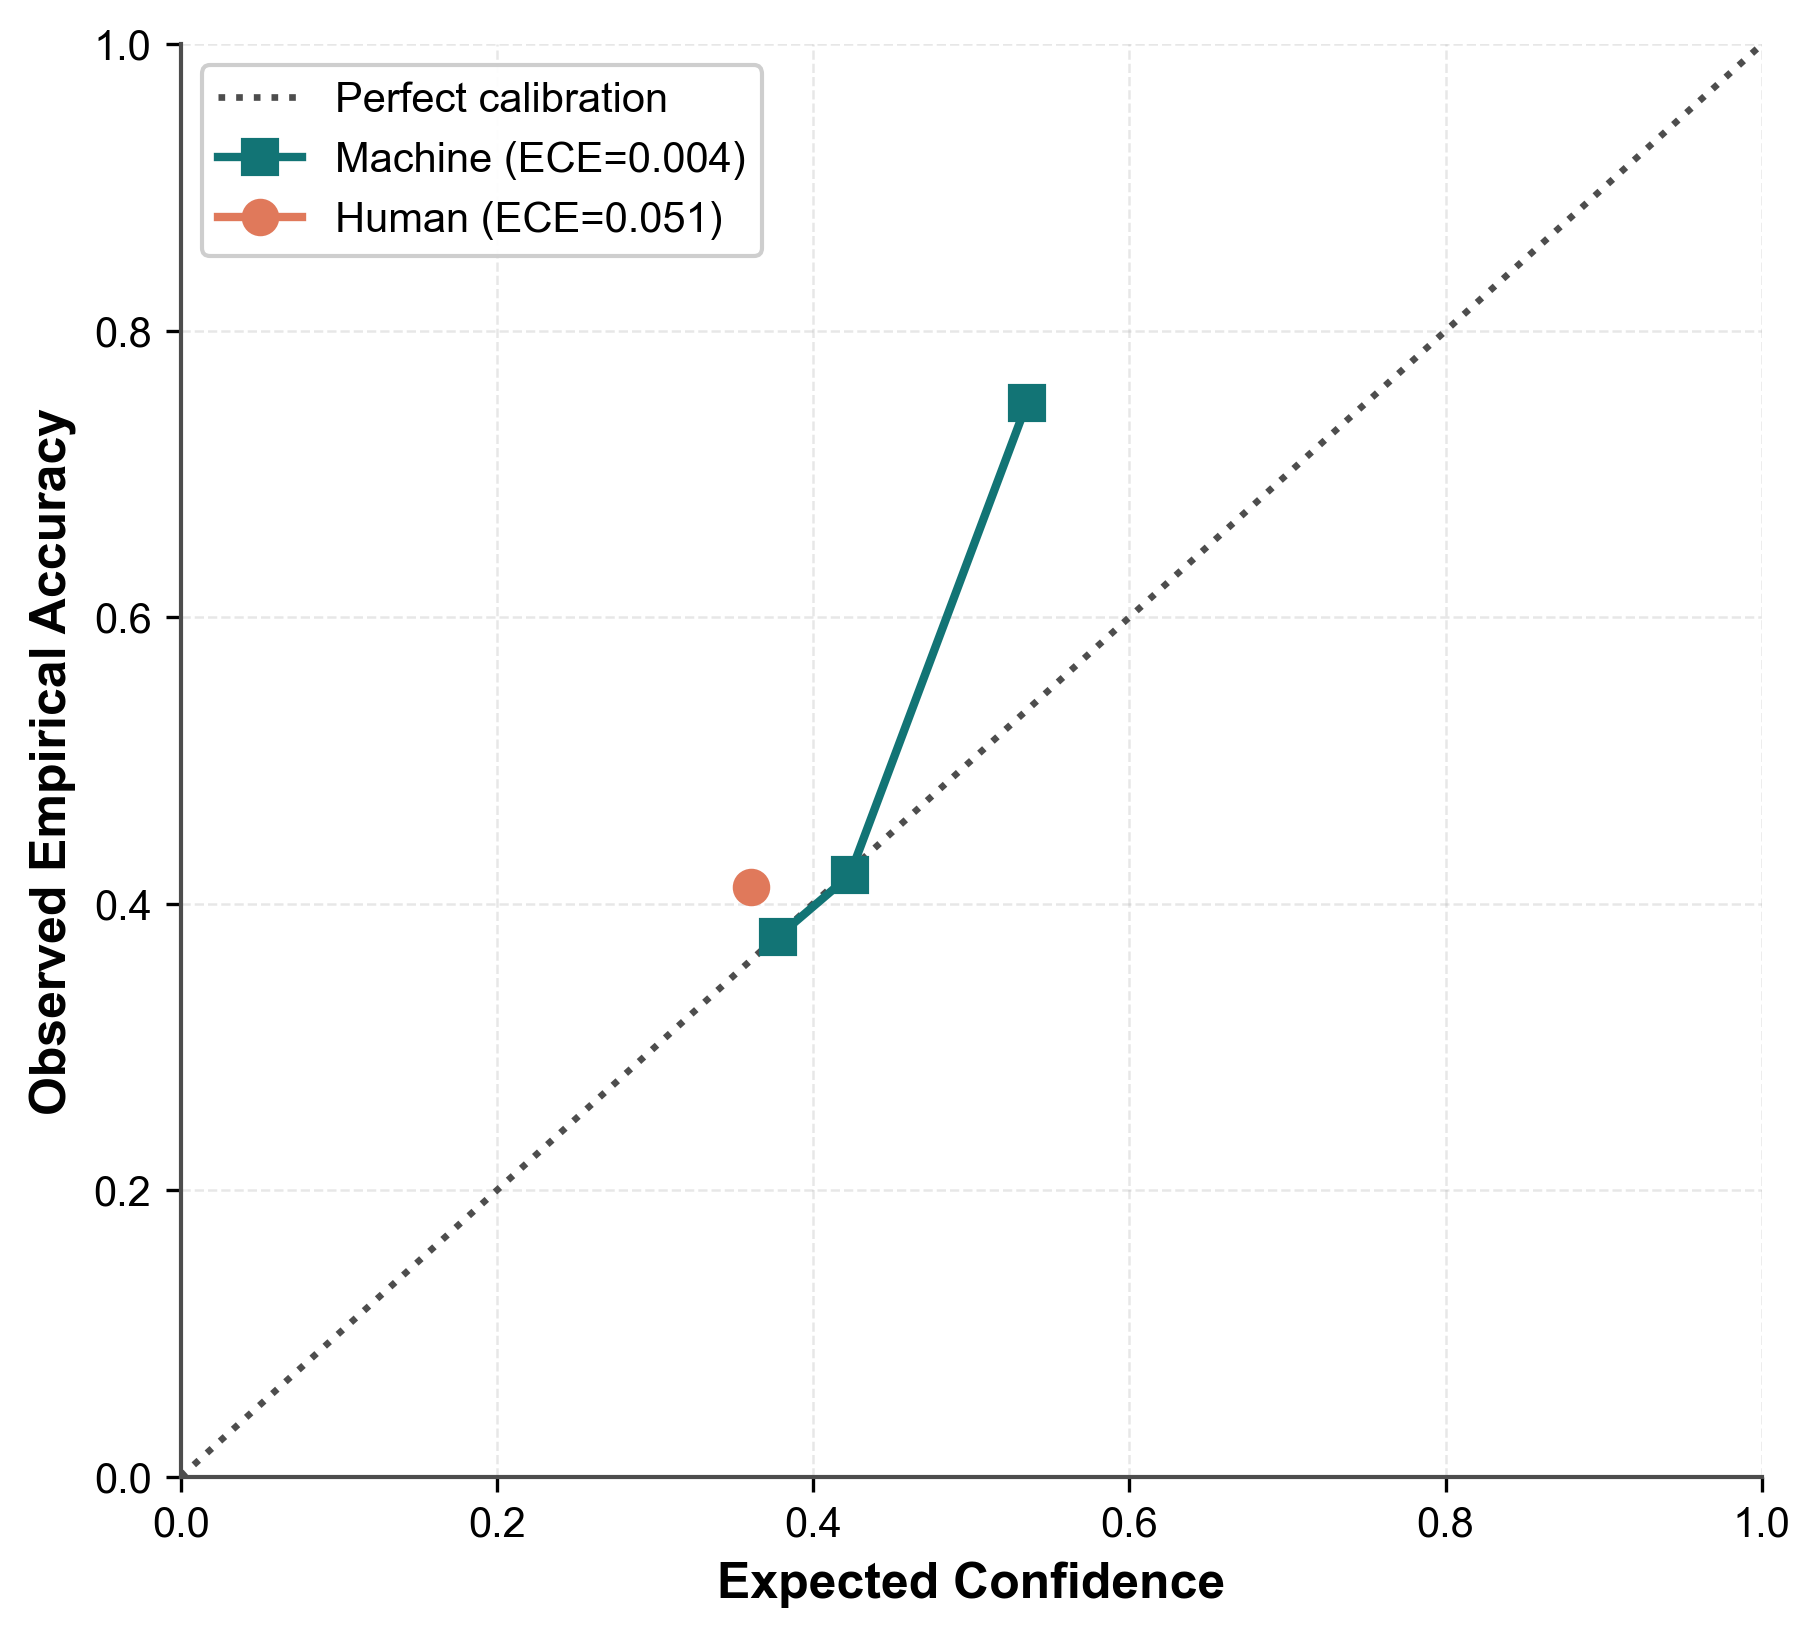
\includegraphics[width=\linewidth]{figures/case_aapl_calibration_reliability.png}
    \caption{Reliability (both pathways).}\label{fig:case_rel}
  \end{subfigure}\\[3pt]
  \begin{subfigure}[t]{0.5\linewidth}\centering
    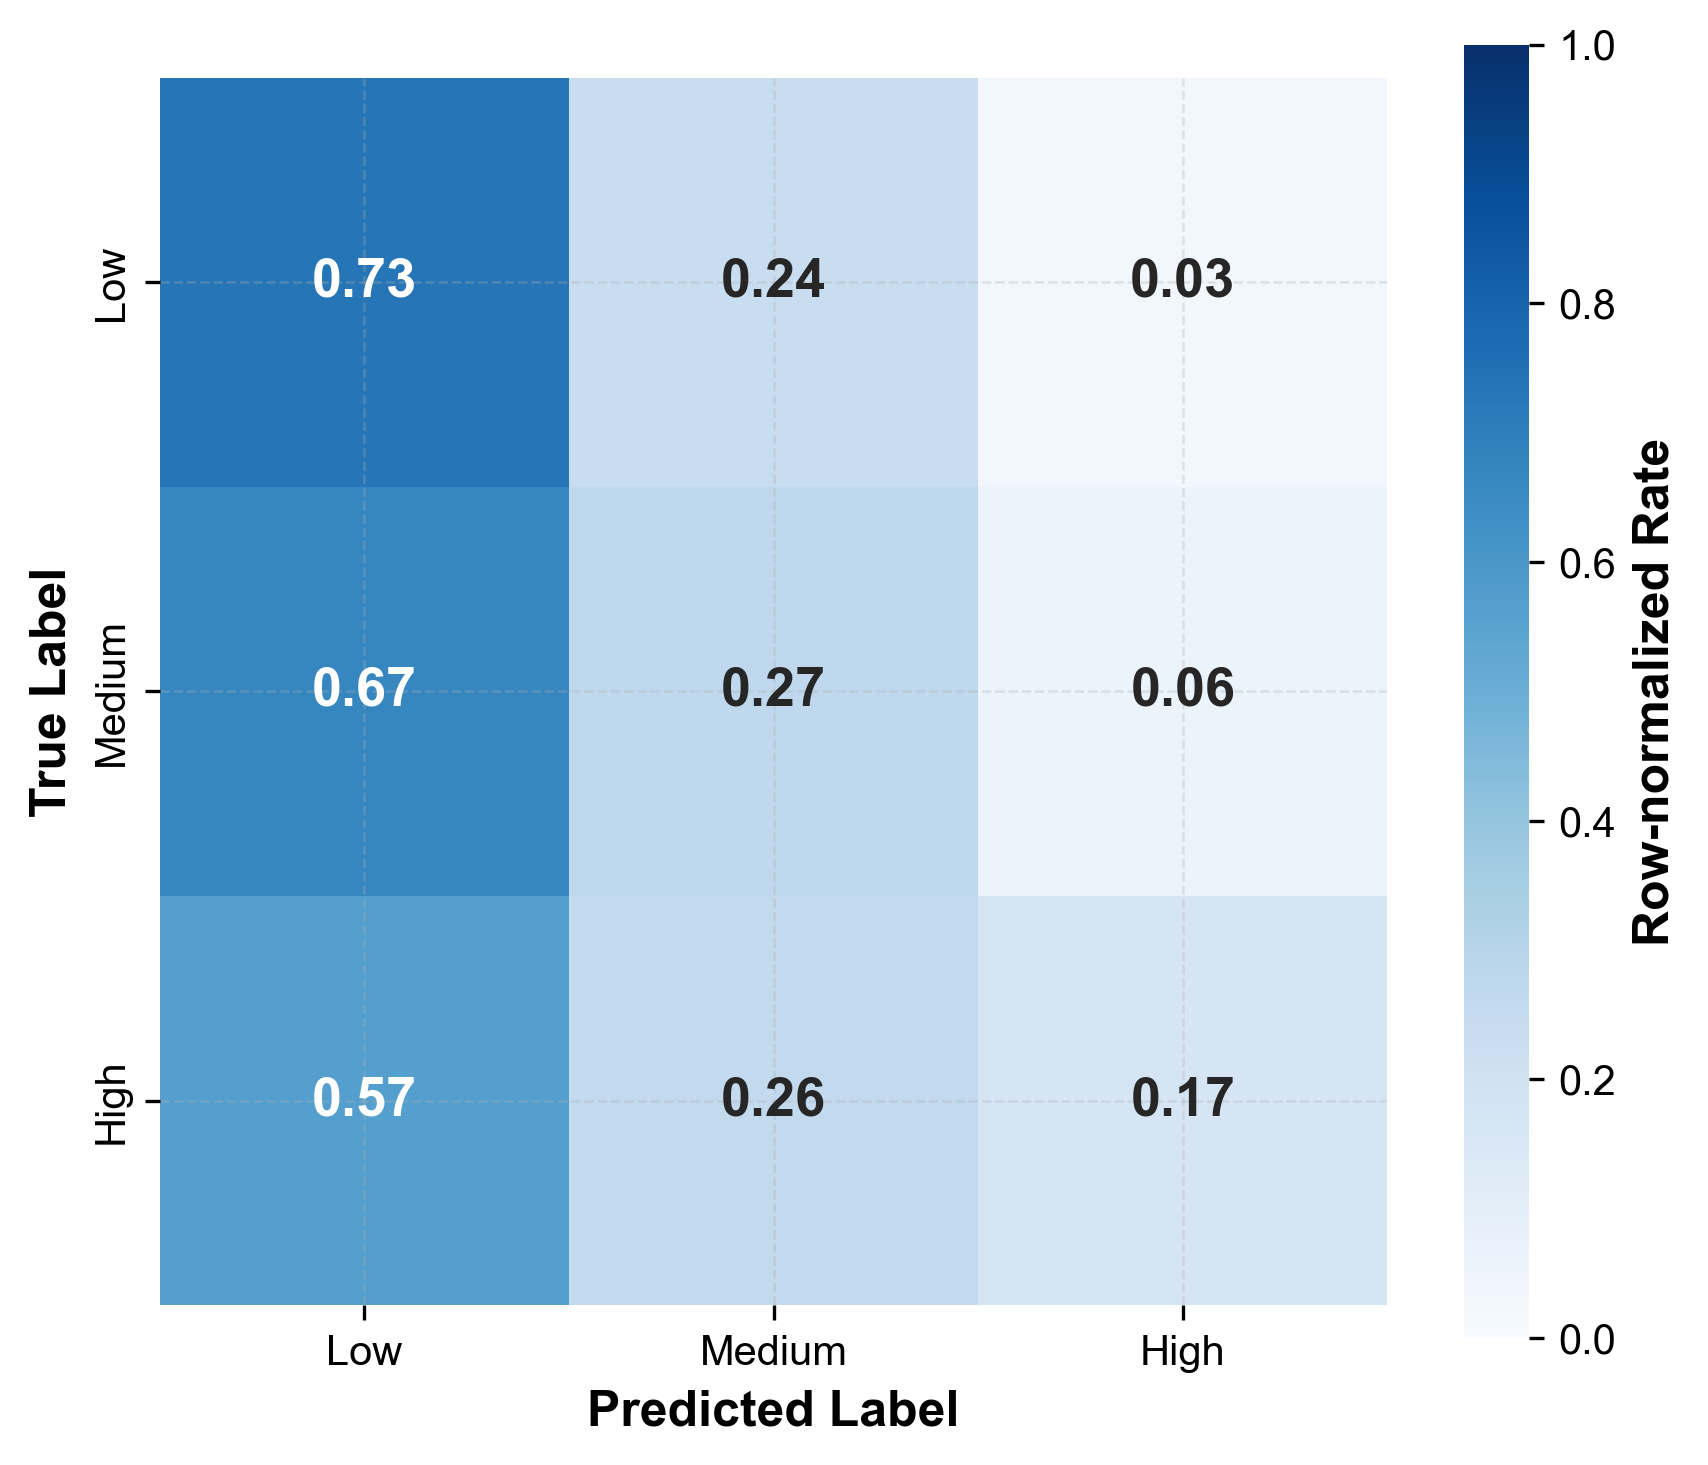
\includegraphics[width=\linewidth]{figures/case_aapl_class_confusion_matrix.png}
    \caption{Machine-pathway confusion matrix (row-normalized).}\label{fig:case_cm}
  \end{subfigure}
  \caption{Bayesian uncertainty, calibration, and error structure on the AAPL
           validation split.}
  \label{fig:case_diag}
\end{figure}

\paragraph{Summary.}
On a real $43$-year AAPL series with intermittent, noisy, drifting supervision,
HINN matches a data-only recurrent baseline in aggregate accuracy
($0.399$ vs.\ $0.409$), improves balanced macro-F1 by $+2.5$ percentage points
through medium-class recovery, remains well-calibrated
($\mathrm{ECE}=0.004$), and exhibits a stable, interpretable trust schedule. The
study substantiates the framework's robustness claims on authentic
non-stationary data while transparently bounding predictive performance: absolute
accuracy is modest, $\mathrm{AUC}_{\mathrm{ovo}}\approx 0.54$, and high-volatility
recall remains the principal target for future improvement.
